\documentclass{fenicscourse}

\begin{document}

\fenicslecture{Lecture 0: Introduction to FEM}
              {Anders Logg}

\linespread{1.5}

\begin{frame}
  \frametitle{What is FEM?}

  \emph{The finite element method is a framework and a recipe for
    discretization of differential equations}

  \begin{itemize}
  \item
    Ordinary differential equations
  \item
    Partial differential equations
  \item
    Integral equations
  \end{itemize}

  \begin{itemize}
  \item
    A recipe for discretization of PDE
  \item
    PDE $\rightarrow$ $Ax = b$
  \item
    Different bases, stabilization, error control, adaptivity
  \end{itemize}

\end{frame}

\begin{frame}
  \frametitle{The FEM cookbook}

  \def\svgwidth{1.05\textwidth}
  \import{pdf/}{pdf/fem_steps.pdf_tex}

\end{frame}

\begin{frame}
  \frametitle{The PDE (i)}

  Consider Poisson's equation, the Hello World of partial differential
  equations:
  \begin{equation*}
    \begin{split}
      - \Delta u &= f \,\,\, \quad \mbox{in } \Omega
      \\
    u &= u_0 \quad \mbox{on } \partial \Omega
    \end{split}
  \end{equation*}

  Poisson's equation arises in numerous applications:
  \begin{itemize}
  \item
    heat conduction, electrostatics, diffusion
    of substances, twisting of elastic rods, inviscid fluid flow, water
    waves, magnetostatics, \ldots
  \item
    as part of numerical splitting strategies for more complicated
    systems of PDEs, in particular the Navier--Stokes equations
  \end{itemize}

\end{frame}

\begin{frame}
  \frametitle{From PDE (i) to variational problem (ii)}

  The simple recipe is: multiply the PDE by a test function $v$ and
  integrate over $\Omega$:
  \begin{equation*}
    -\int_\Omega (\Delta u)v \dx = \int_\Omega fv\dx
  \end{equation*}

  Then integrate by parts and set $v = 0$ on the Dirichlet boundary:

  \begin{equation*}
    -\int_\Omega (\Delta u) v \dx
    = \int_\Omega \nabla u\cdot\nabla v\dx -
   \underbrace{\int_{\partial\Omega} \frac{\partial u}{\partial n} v\ds}_{\textcolor{fenicsred}{=0}}
  \end{equation*}

  We find that:
  \begin{equation*}
    \int_\Omega\nabla u\cdot\nabla v\dx = \int_\Omega fv\dx
  \end{equation*}

\end{frame}

\begin{frame}
  \frametitle{The variational problem (ii)}

  Find $u \in V$ such that
  \begin{equation*}
    \int_{\Omega} \nabla u \cdot \nabla v \dx =
    \int_{\Omega} fv \dx
  \end{equation*}
  for all $v \in \hat{V}$

  \bigskip

  The trial space $V$ and the test space $\hat{V}$ are (here)
  given by
  \begin{equation*}
    \begin{split}
      V       &= \{v \in H^1(\Omega) : v = u_0 \mbox{ on } \partial\Omega\} \\
      \hat{V} &= \{v \in H^1(\Omega) : v = 0 \mbox{ on } \partial\Omega\}
    \end{split}
  \end{equation*}

\end{frame}

\begin{frame}
  \frametitle{From continuous (ii) to discrete (iii) problem}

  We approximate the continuous variational problem with a discrete
  variational problem posed on finite dimensional subspaces of $V$ and $\hat{V}$:

  \begin{align*}
    V_h &\subset V \\
    \hat{V}_h &\subset \hat{V}
  \end{align*}

  \bigskip

  Find $u_h \in V_h \subset V$ such that
  \begin{equation*}
    \int_{\Omega} \nabla u_h \cdot \nabla v \dx =
    \int_{\Omega} fv \dx
  \end{equation*}
  for all $v \in \hat{V}_h \subset \hat{V}$

\end{frame}

\begin{frame}
  \frametitle{From discrete variational problem (iii) to discrete
    system of equations (iv)}

  Choose a basis for the discrete function space:
  \begin{equation*}
    V_h = \mathrm{span} \, \{\phi_j\}_{j=1}^N
  \end{equation*}

  Make an ansatz for the discrete solution:
  \begin{equation*}
    u_h = \sum_{j=1}^N U_j \phi_j
  \end{equation*}

  Test against the basis functions:
  \begin{equation*}
    \int_{\Omega} \nabla
    (\underbrace{\sum_{j=1}^N U_j \phi_j}_{\textcolor{red}{u_h}})
    \cdot \nabla \phi_i \dx = \int_{\Omega} f \phi_i \dx
  \end{equation*}

\end{frame}

\begin{frame}
  \frametitle{From discrete variational problem (iii) to discrete
    system of equations (iv), cont'd.}

  Rearrange to get:
  \begin{equation*}
    \sum_{j=1}^N U_j
    \underbrace{\int_{\Omega} \nabla \phi_j \cdot
      \nabla \phi_i \dx}_{\textcolor{red}{A_{ij}}}
    = \underbrace{\int_{\Omega} f\phi_i \dx}_{\textcolor{red}{b_i}}
  \end{equation*}

  A linear system of equations:
  \begin{equation*}
    A U = b
  \end{equation*}
  where
  \begin{align}
    A_{ij} &= \int_{\Omega} \nabla \phi_j \cdot \nabla \phi_i \dx \\
    b_i   &= \int_{\Omega} f\phi_i \dx
  \end{align}

\end{frame}

\begin{frame}
  \frametitle{The canonical abstract problem}

  (i) Partial differential equation:
  \begin{equation*}
    \mathcal{A} u = f \quad \text{ in } \Omega
  \end{equation*}

  (ii) Continuous variational problem: find $u \in V$ such that
  \begin{equation*}
    a(u, v) = L(v) \quad \text{ for all } v \in \hat{V}
  \end{equation*}

  (iii) Discrete variational problem: find $u_h \in V_h \subset
  V$ such that
  \begin{equation*}
    a(u_h, v) = L(v) \quad \text{ for all } v \in \hat{V}_h
  \end{equation*}

  (iv) Discrete system of equations for $u_h = \sum_{j=1}^N
  U_j \phi_j$:
  \begin{align*}
    A U &= b \\
    A_{ij} &= a(\phi_j, \phi_i) \\
    b_i   &= L(\phi_i)
  \end{align*}

\end{frame}

\begin{frame}
  \frametitle{Important topics}

  \begin{itemize}
  \item
    \emph{How to choose $V_h$?}
  \item
    \emph{How to compute $A$ and $b$}
  \item
    \emph{How to solve $AU = b$?}
  \item
    \emph{Can we quantify/control How large the error $e = u - u_h$ is?}
  \item
    \emph{Can we assess the cost of solving the system?}
  \item
    \textcolor{grey}{Extensions to nonlinear, time-dependent, complicated problems}
  \end{itemize}

\end{frame}


\fenicssection{How to choose $V_h$}

\begin{frame}
  \frametitle{Finite element function spaces}

  \begin{center}
    \def\svgwidth{\textwidth}
    \import{pdf/}{pdf/lin.pdf_tex}
  \end{center}

\end{frame}

\begin{frame}
  \frametitle{The finite element definition (Ciarlet 1975)}

  A finite element is a triple $(T, \mathcal{V}, \mathcal{L})$, where
  \begin{itemize}
  \item
    the domain $T$ is a bounded, closed subset of $\R^d$ (for $d = 1,
    2, 3, \dots$) with nonempty interior and piecewise smooth
    boundary
  \item
    the space $\mathcal{V} = \mathcal{V}(T)$ is a finite
    dimensional function space on $T$ of dimension $n$
  \item
    the set of degrees of freedom (nodes) $\mathcal{L} = \{\ell_1,
    \ell_2,\ldots, \ell_{n}\}$ is a basis for the dual space
    $\mathcal{V}'$; that is, the space of bounded linear functionals
    on $\mathcal{V}$
  \end{itemize}

\end{frame}

\begin{frame}
  \frametitle{The finite element definition (Ciarlet 1975)}

  \def\svgwidth{1.2\textwidth}
  \import{pdf/}{pdf/ciarlet.pdf_tex}

\end{frame}

\begin{frame}
  \frametitle{The linear Lagrange element: $(T, \mathcal{V}, \mathcal{L})$}

  \begin{itemize}
  \item
    $T$ is a line, triangle or tetrahedron
  \item
    $\mathcal{V}$ is the first-degree polynomials on $T$
  \item
    $\mathcal{L}$ is point evaluation at the vertices
  \end{itemize}

\end{frame}

\begin{frame}
  \frametitle{The linear Lagrange element: $\mathcal{L}$}

  \begin{center}
    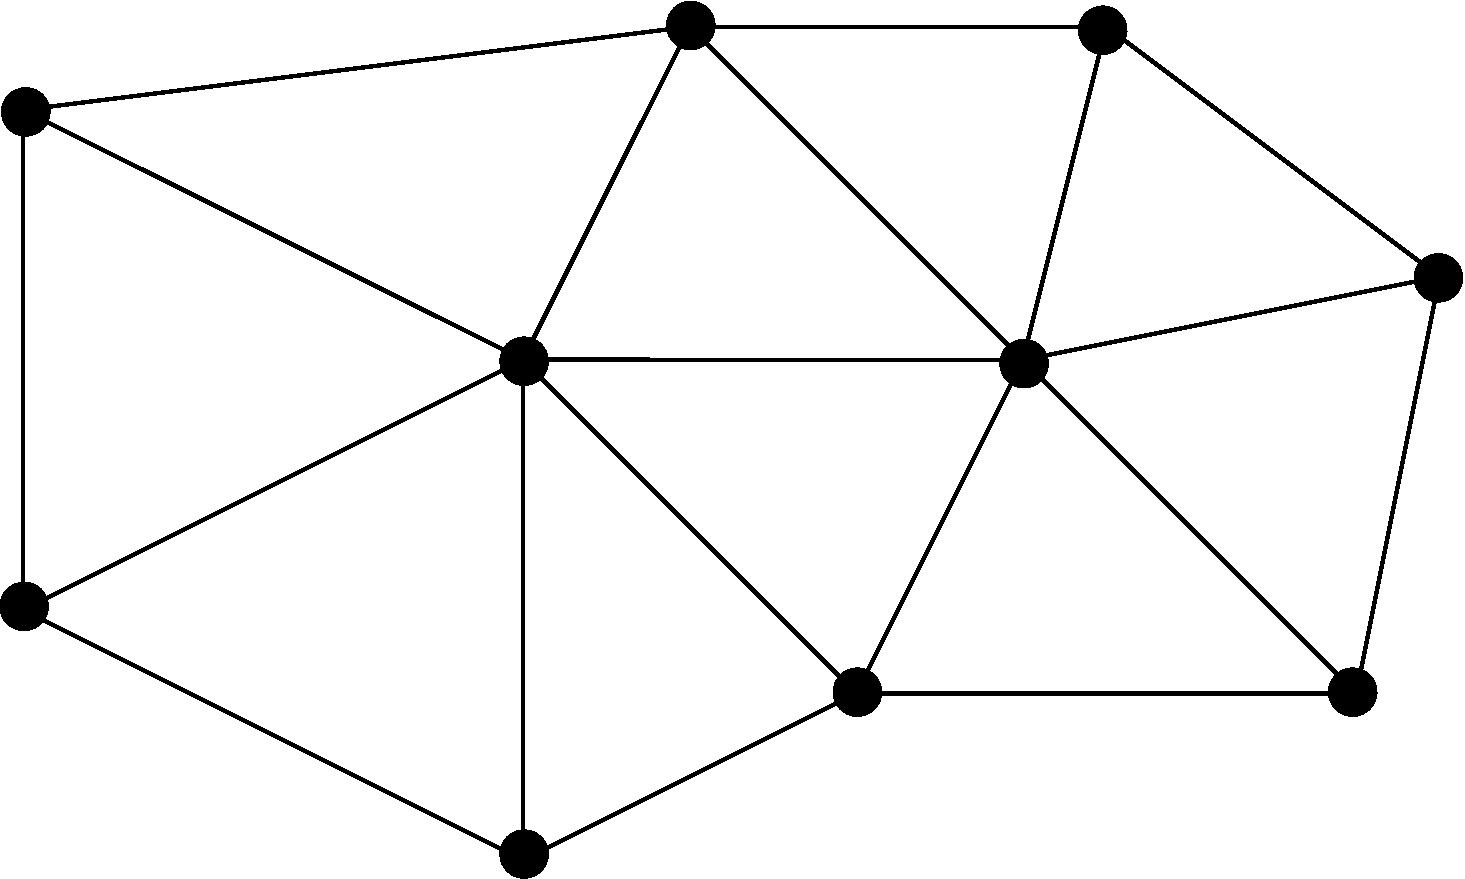
\includegraphics[width=\textwidth]{pdf/mesh-p1.pdf}
  \end{center}

\end{frame}

\begin{frame}
  \frametitle{The linear Lagrange element: $V_h$}

  \begin{center}
    \def\svgwidth{0.8\textwidth}
    \import{pdf/}{pdf/tri.pdf_tex}
  \end{center}

\end{frame}

\begin{frame}
  \frametitle{The quadratic Lagrange element: $(T, \mathcal{V}, \mathcal{L})$}

  \begin{itemize}
  \item
    $T$ is a line, triangle or tetrahedron
  \item
    $\mathcal{V}$ is the second-degree polynomials on $T$
  \item
    $\mathcal{L}$ is point evaluation at the vertices and edge midpoints
  \end{itemize}

\end{frame}

\begin{frame}
  \frametitle{The quadratic Lagrange element: $\mathcal{L}$}

  \begin{center}
    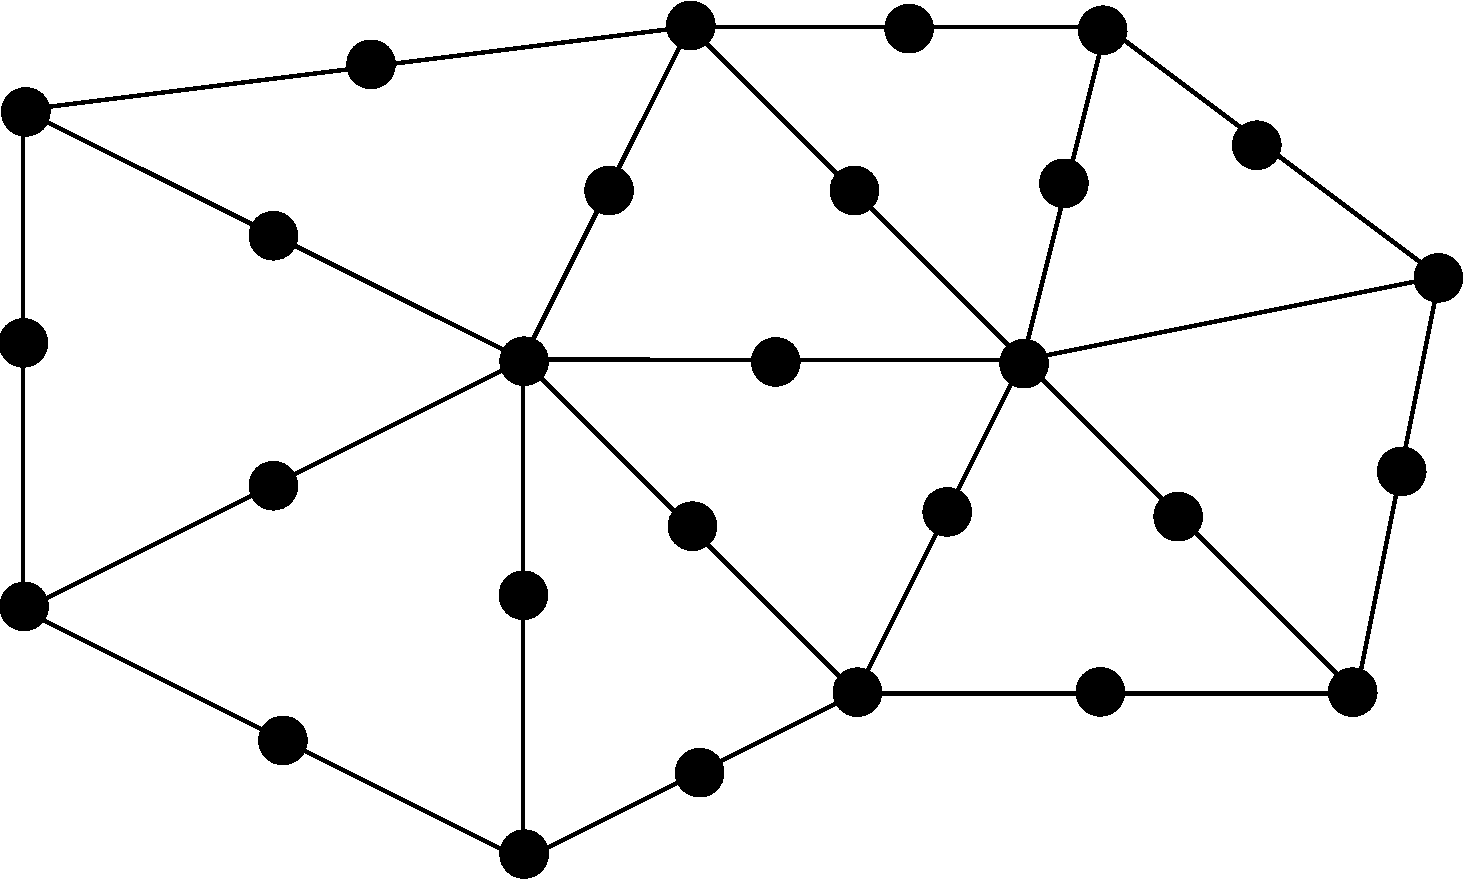
\includegraphics[width=\textwidth]{pdf/mesh-p2.pdf}
  \end{center}

\end{frame}

\begin{frame}
  \frametitle{The quadratic Lagrange element: $V_h$}

  \begin{center}
    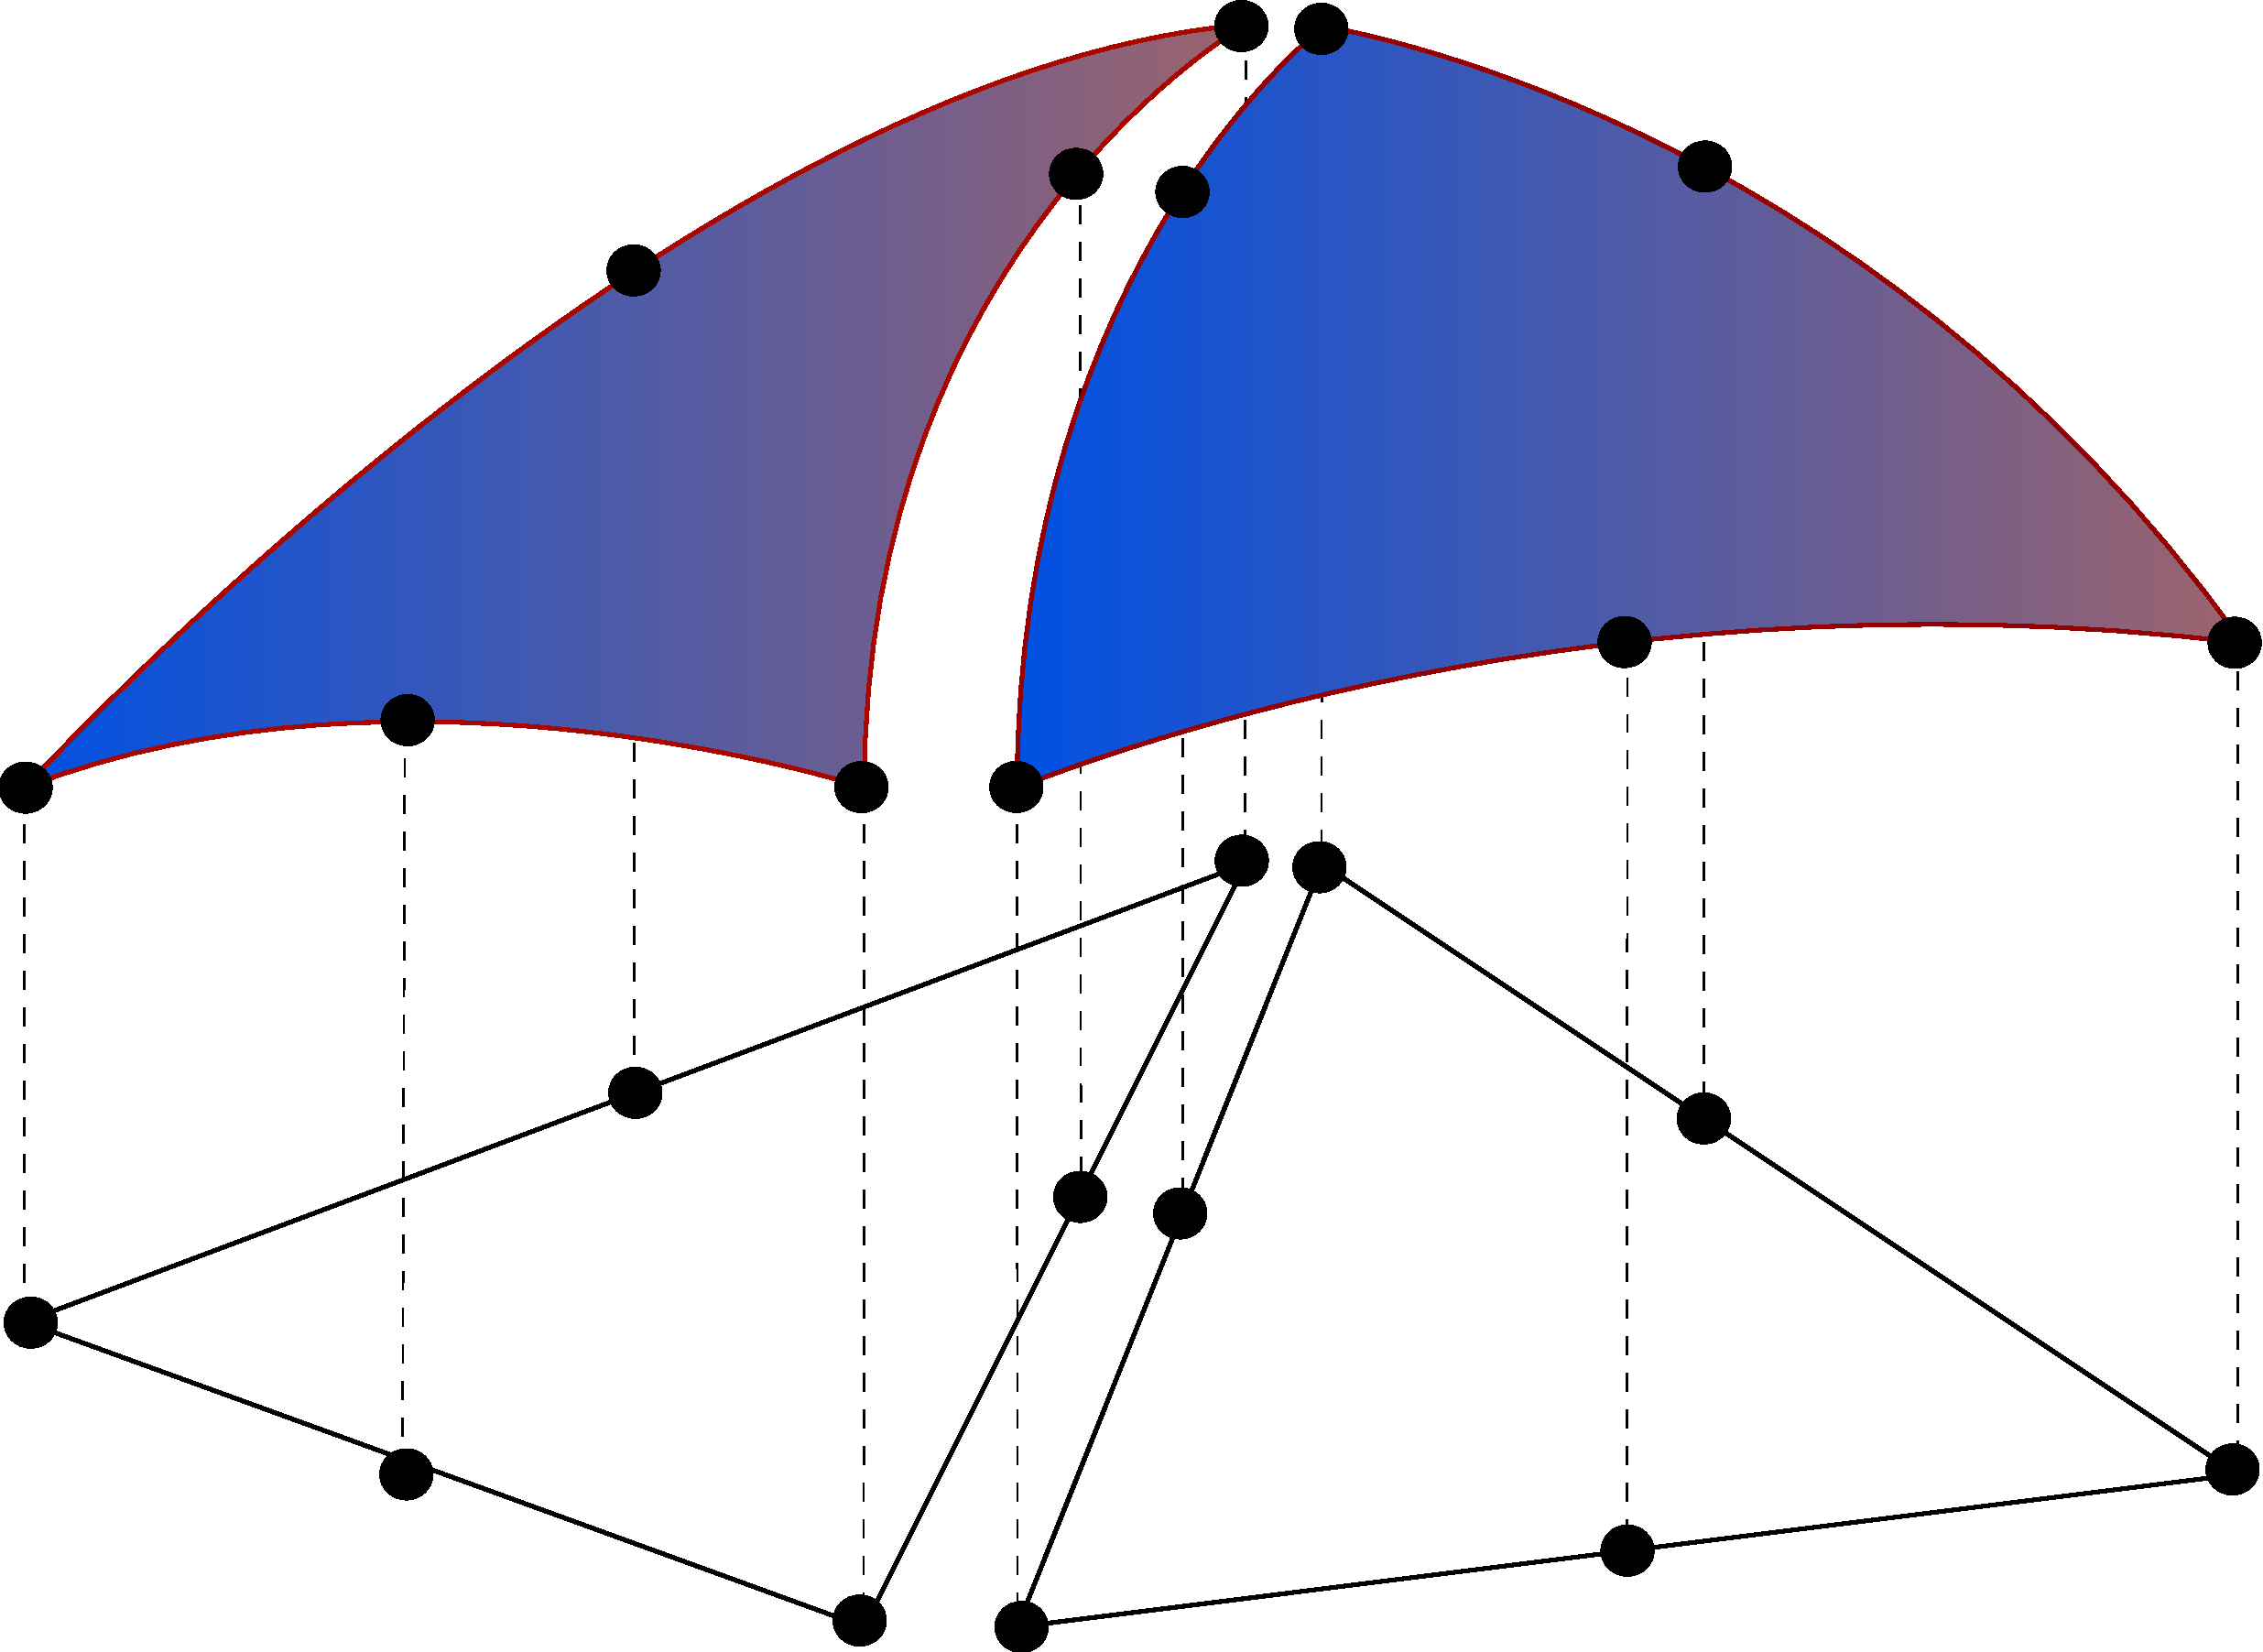
\includegraphics[width=0.9\textwidth]{pdf/femspace.pdf}
  \end{center}

\end{frame}

\begin{frame}
  \frametitle{Families of elements}

  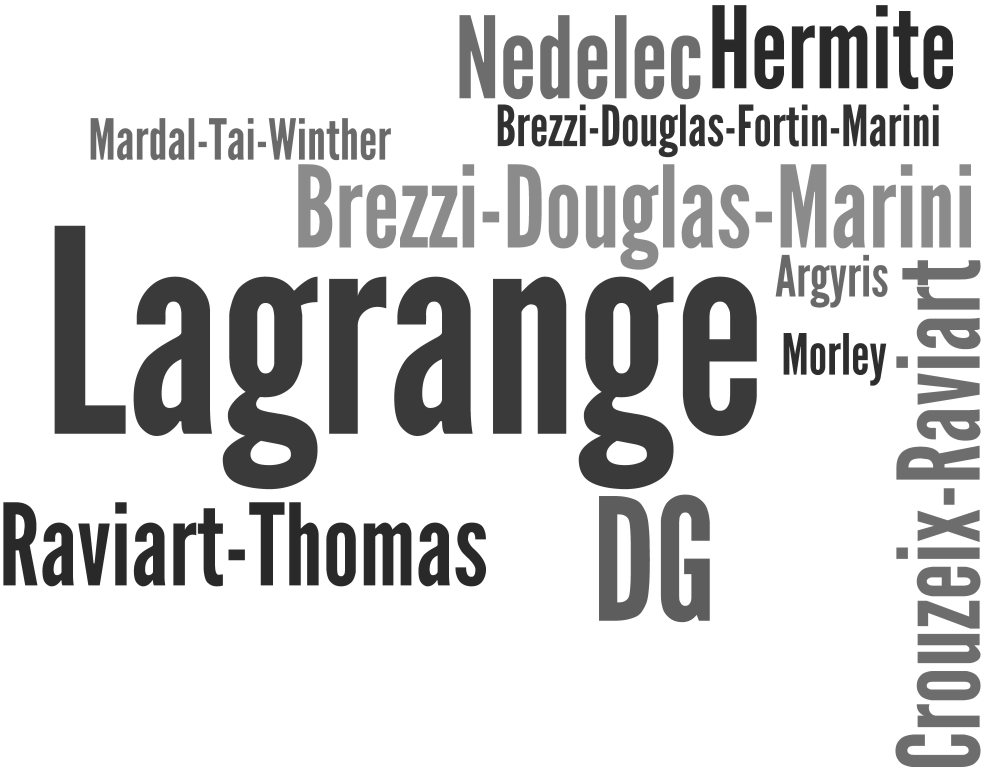
\includegraphics[width=0.9\textwidth]{png/elements_wordle.png}

\end{frame}

\begin{frame}
  \frametitle{Families of elements}

  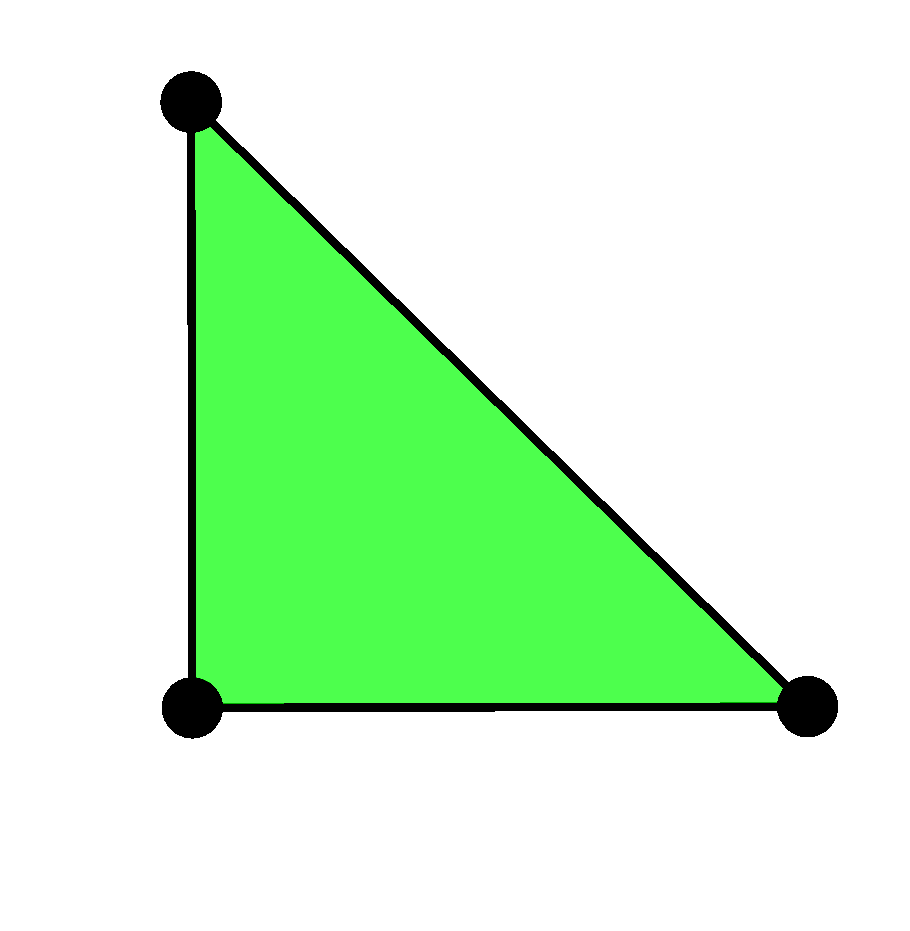
\includegraphics[width=1.3cm]{png/CG1_2d.png}
  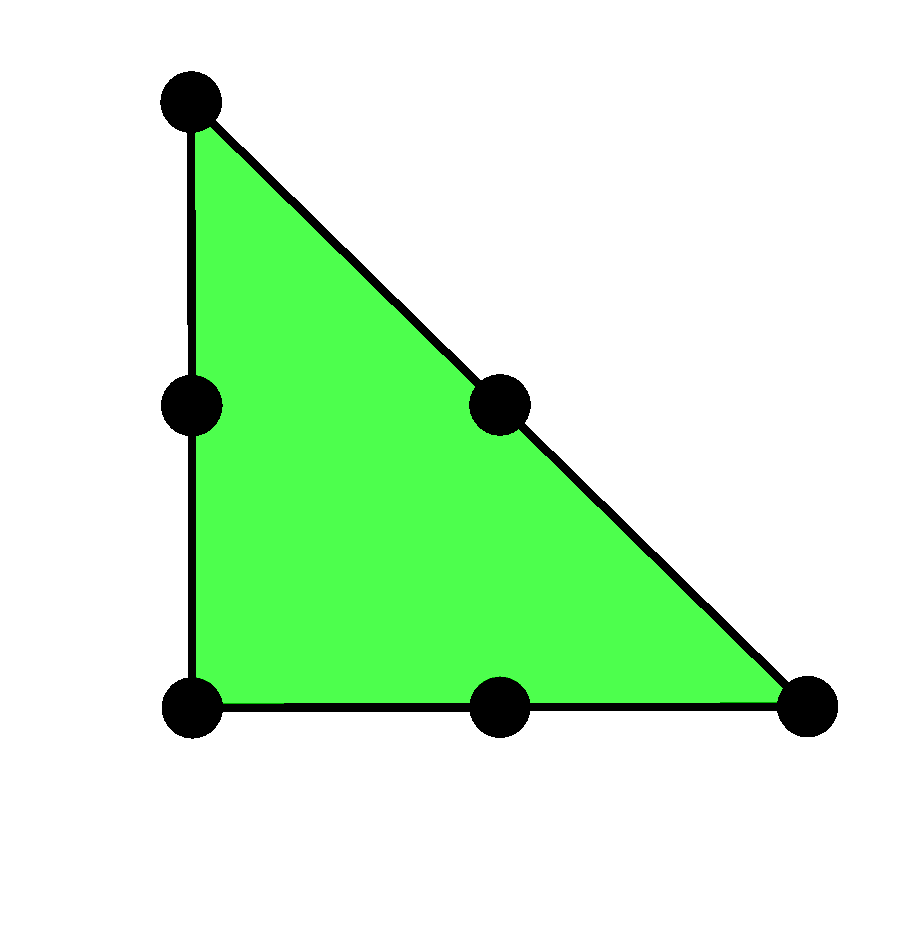
\includegraphics[width=1.3cm]{png/CG2_2d.png}
  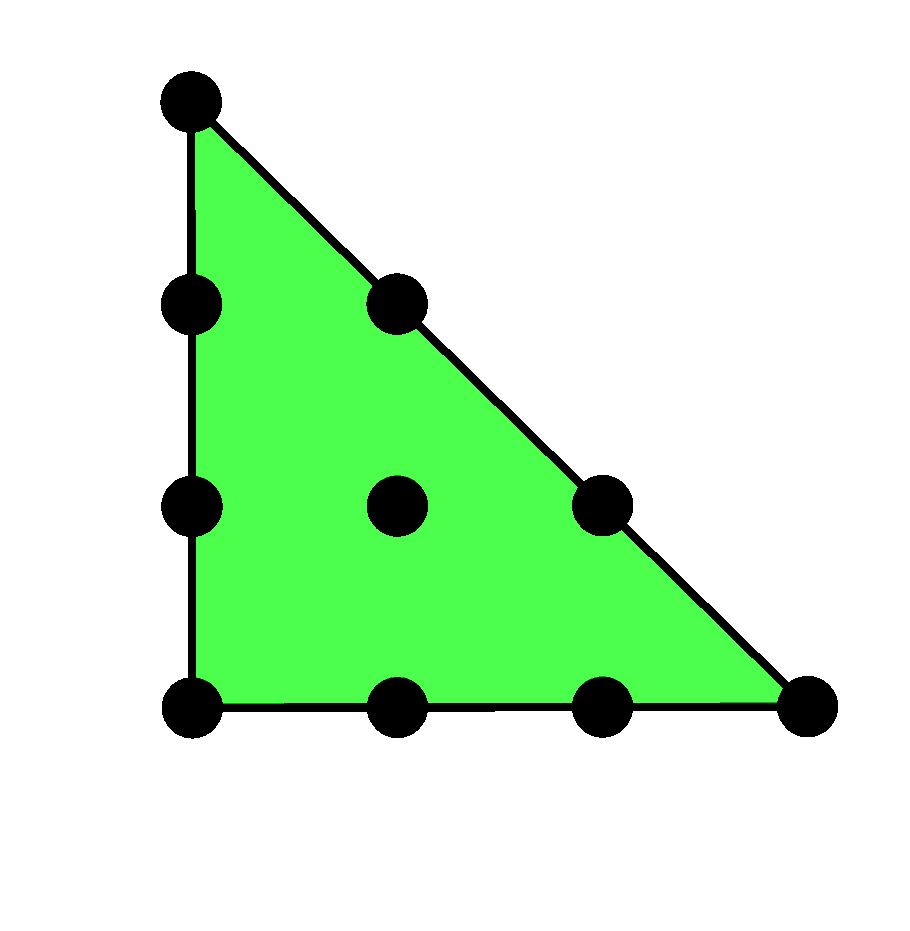
\includegraphics[width=1.3cm]{png/CG3_2d.png}
  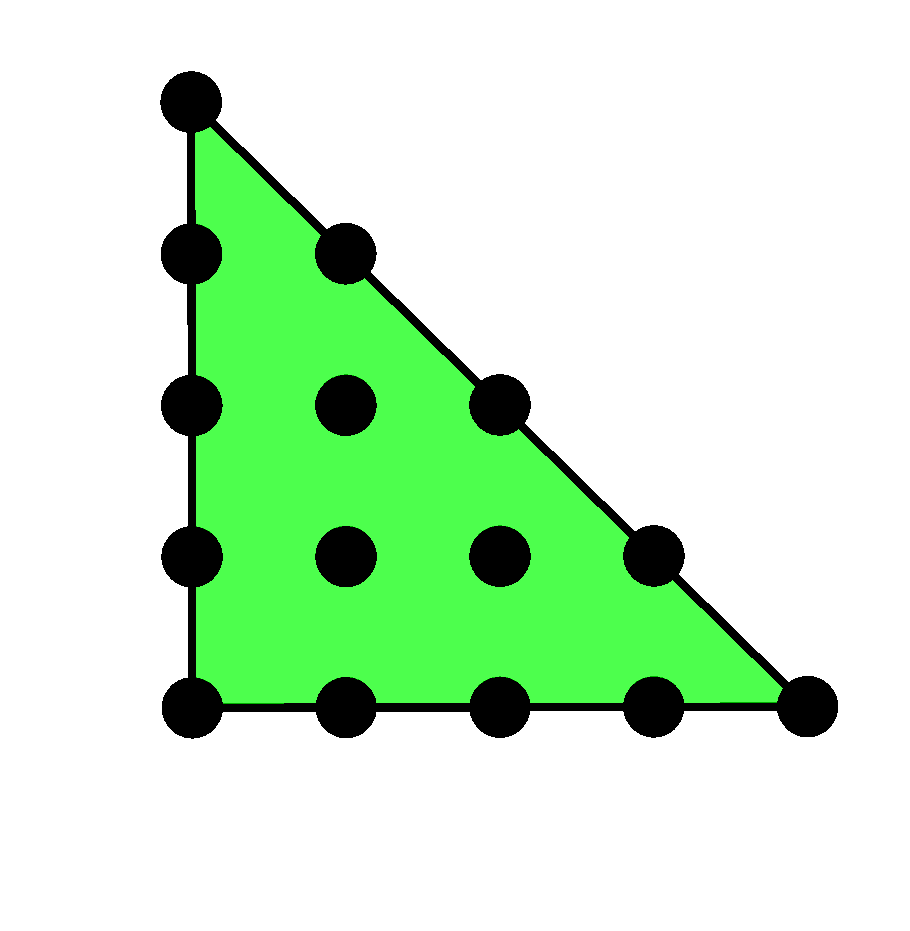
\includegraphics[width=1.3cm]{png/CG4_2d.png}
  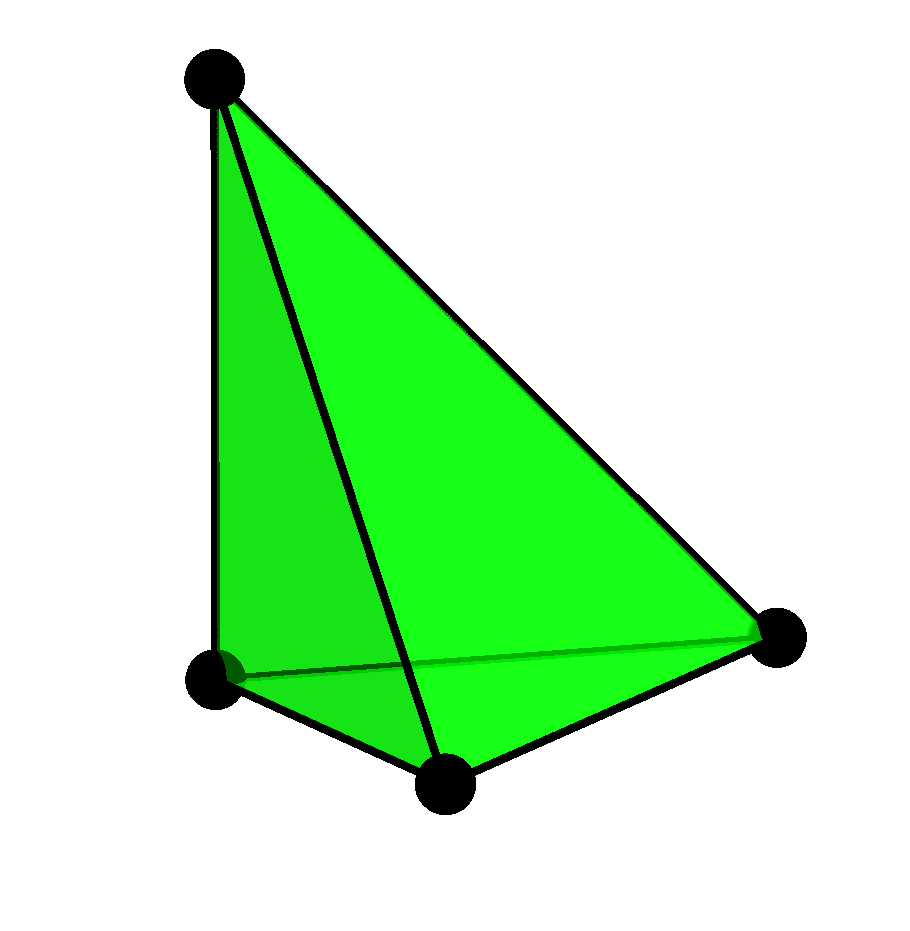
\includegraphics[width=1.3cm]{png/CG1_3d.png}
  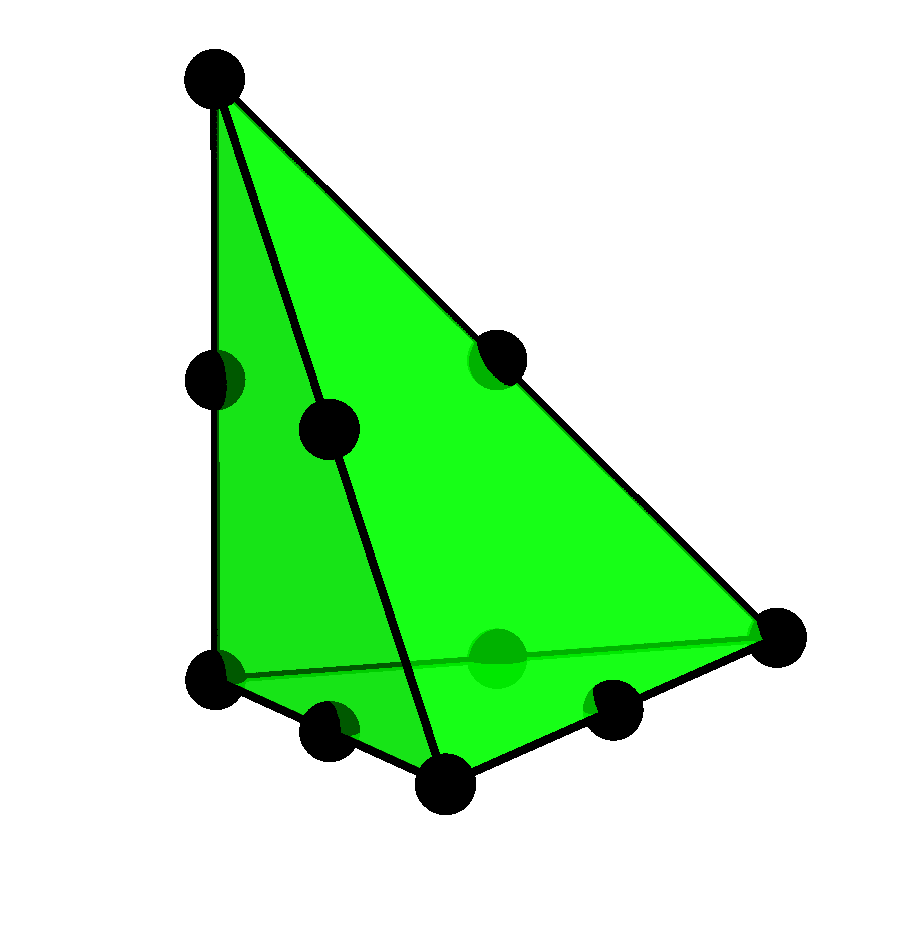
\includegraphics[width=1.3cm]{png/CG2_3d.png}
  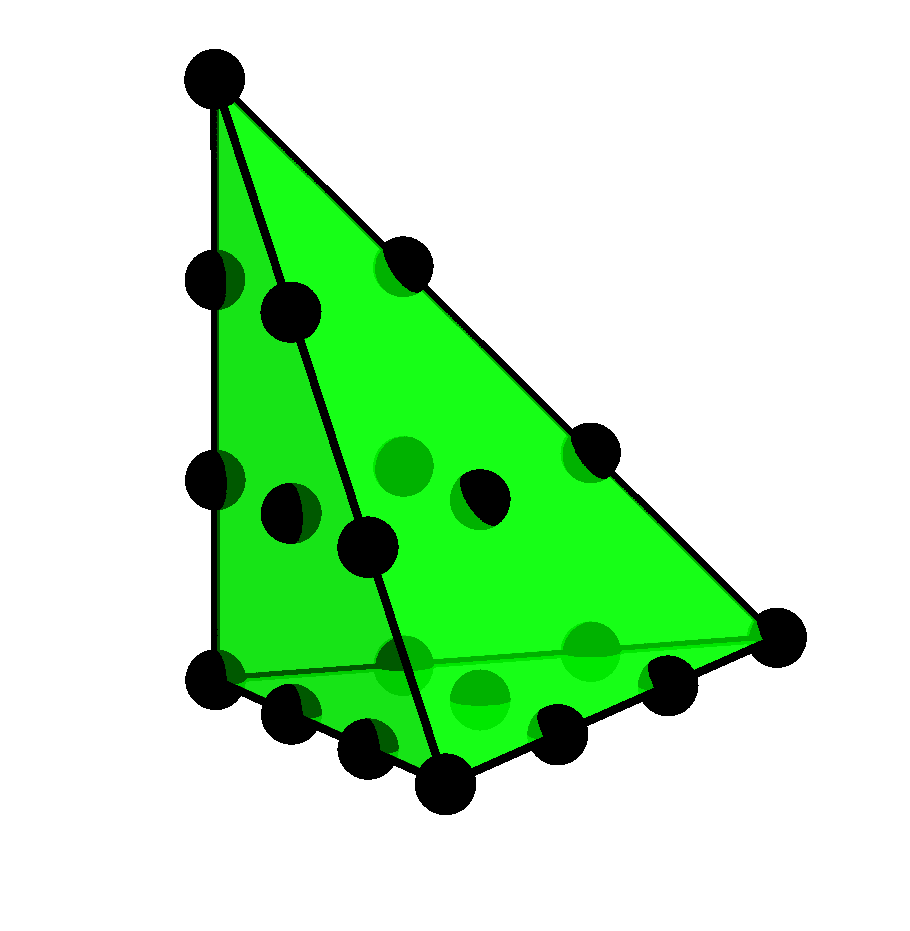
\includegraphics[width=1.3cm]{png/CG3_3d.png}
  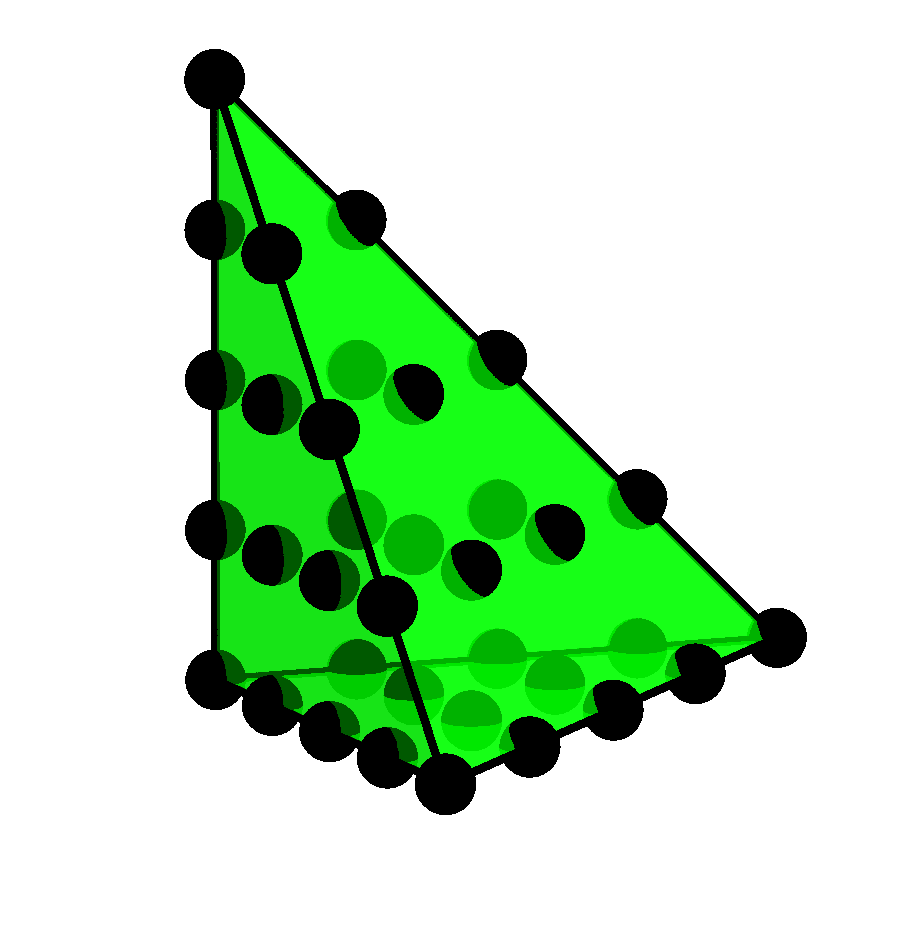
\includegraphics[width=1.3cm]{png/CG4_3d.png} \\
  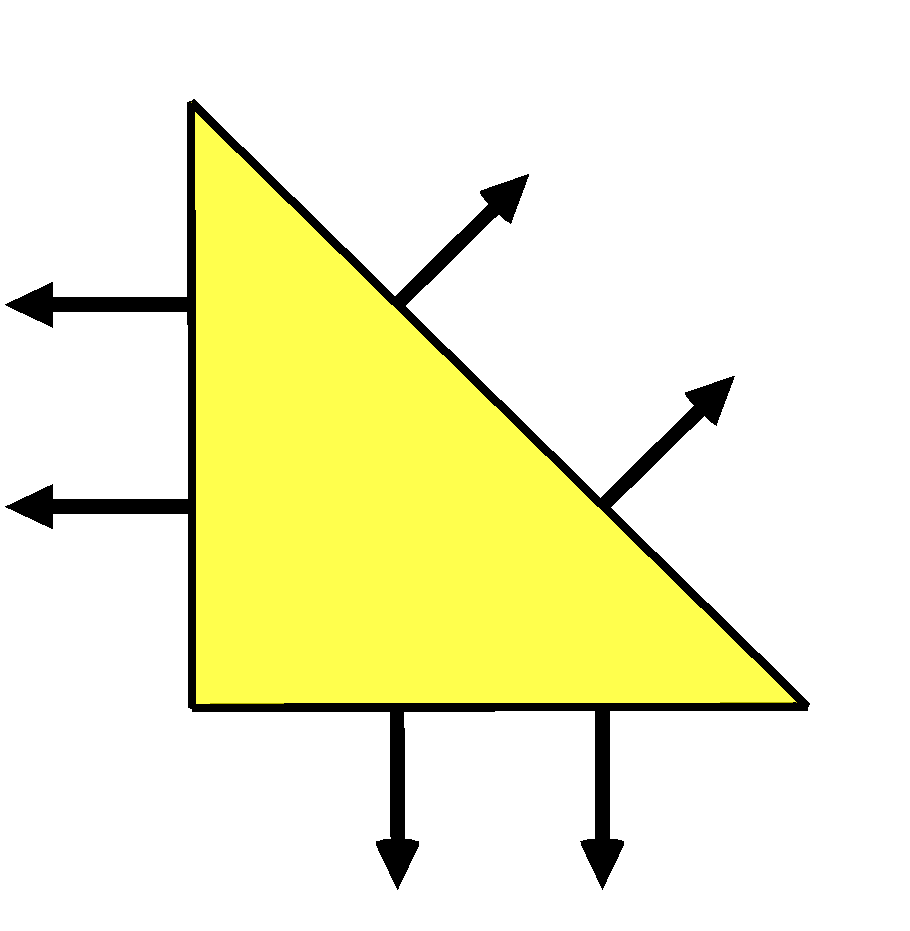
\includegraphics[width=1.3cm]{png/BDM1_2d.png}
  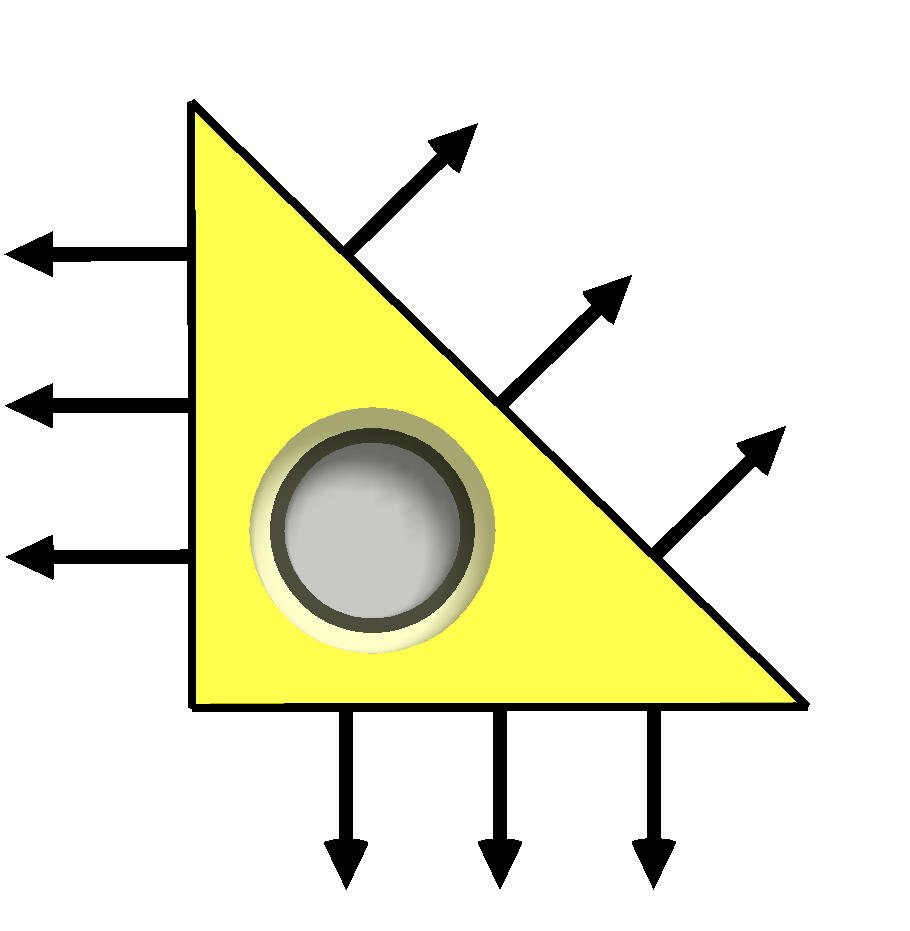
\includegraphics[width=1.3cm]{png/BDM2_2d.png}
  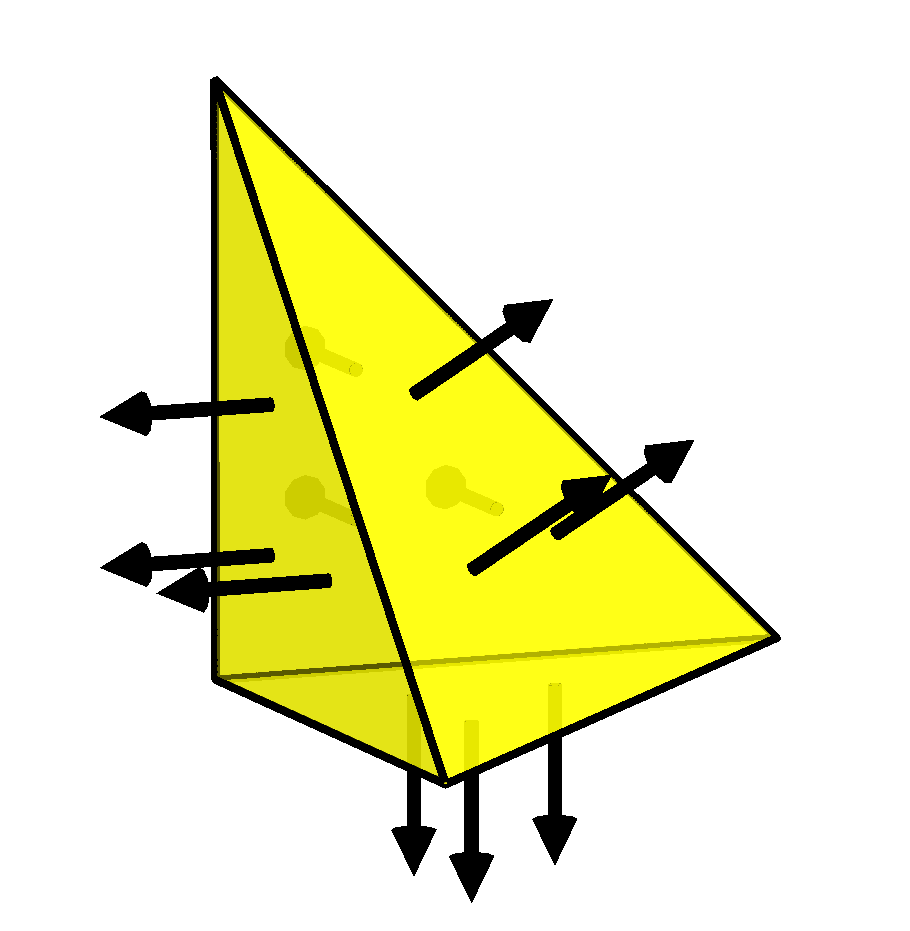
\includegraphics[width=1.3cm]{png/BDM1_3d.png}
  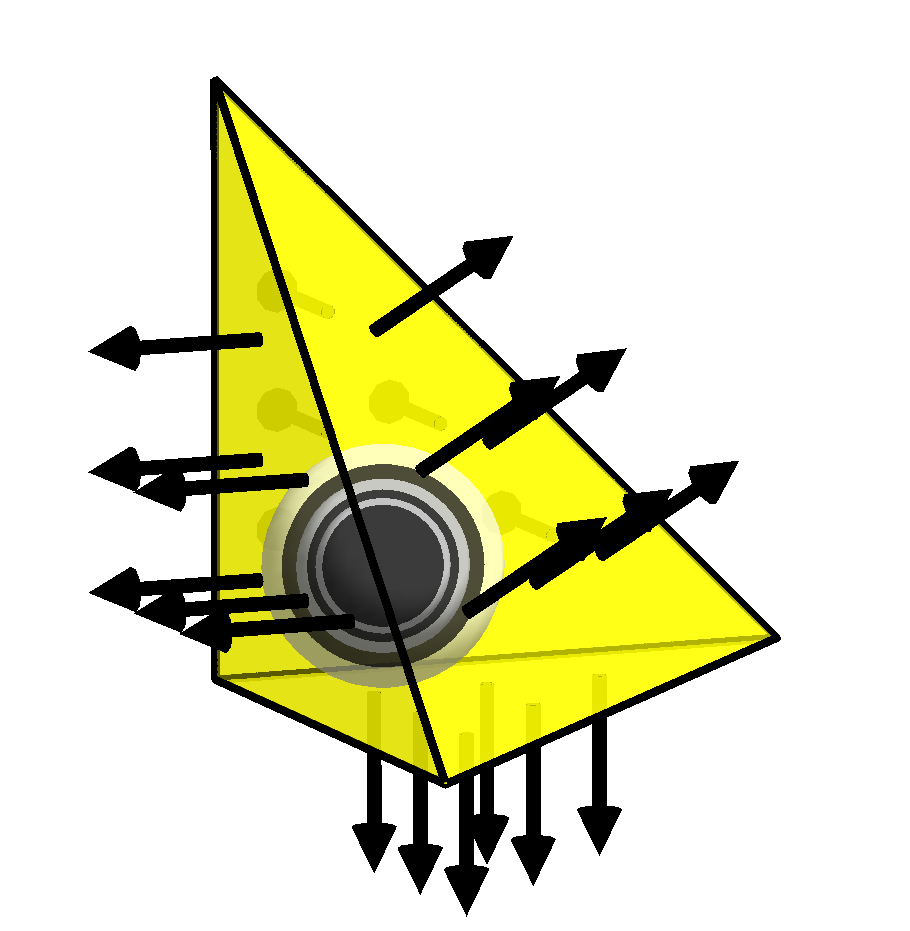
\includegraphics[width=1.3cm]{png/BDM2_3d.png}
  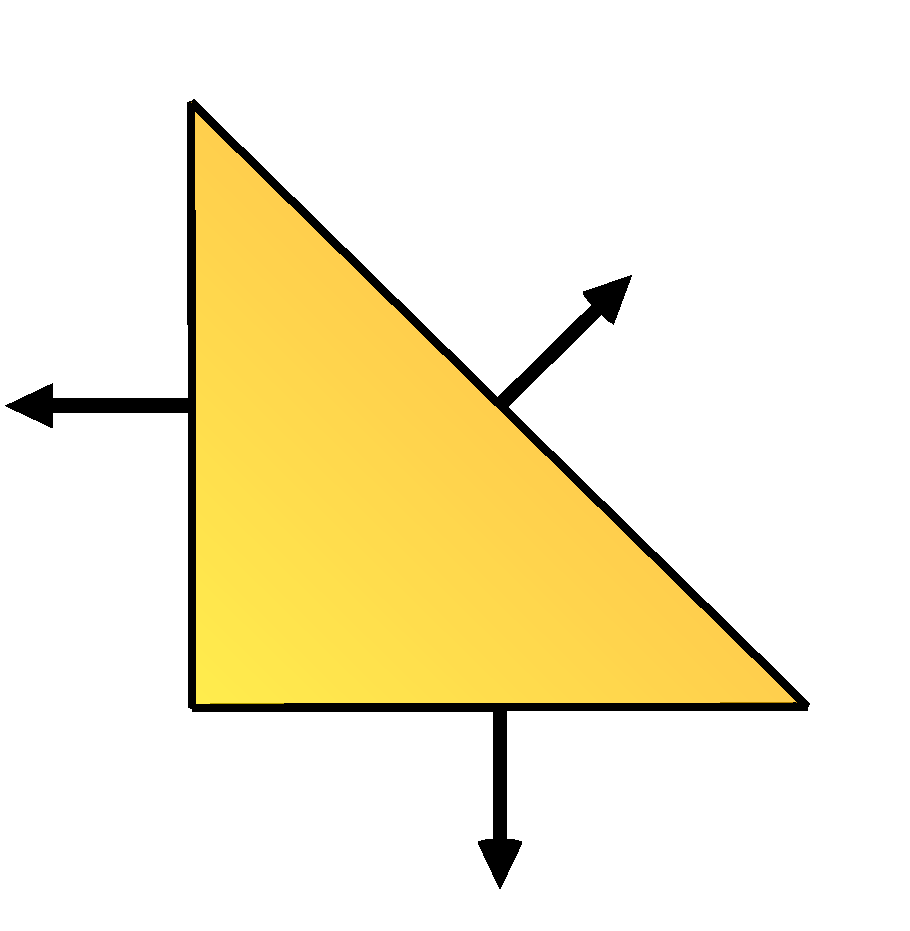
\includegraphics[width=1.3cm]{png/RT1_2d.png}
  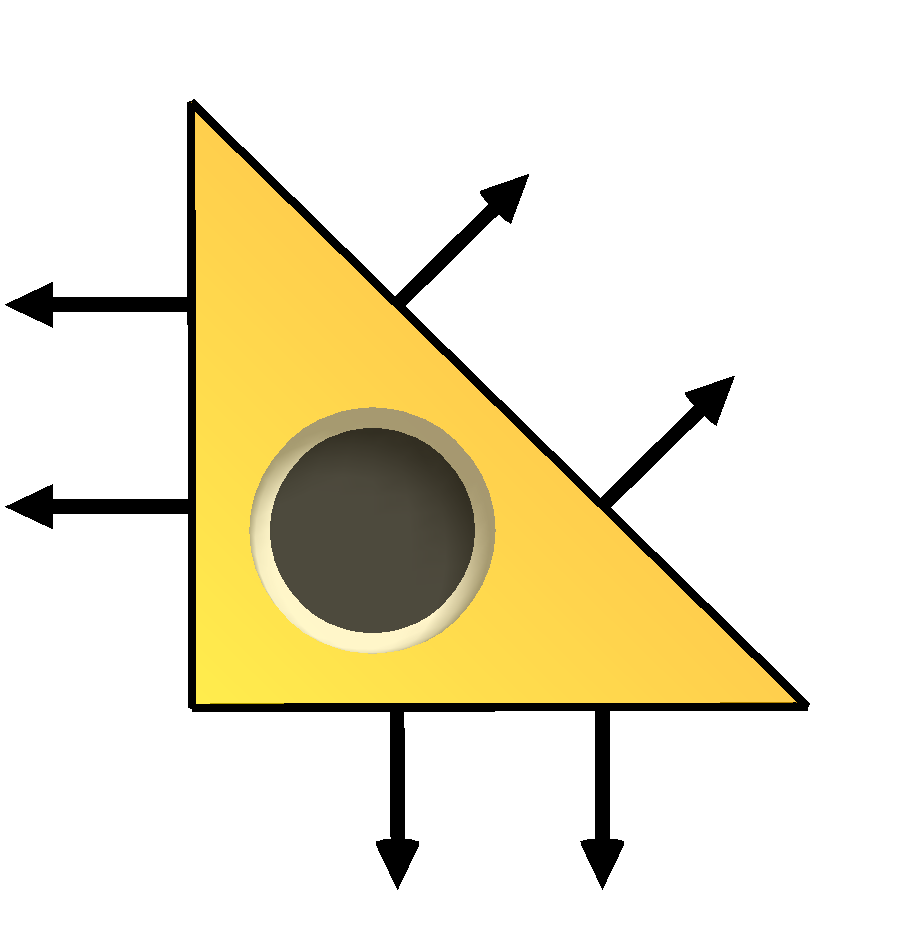
\includegraphics[width=1.3cm]{png/RT2_2d.png}
  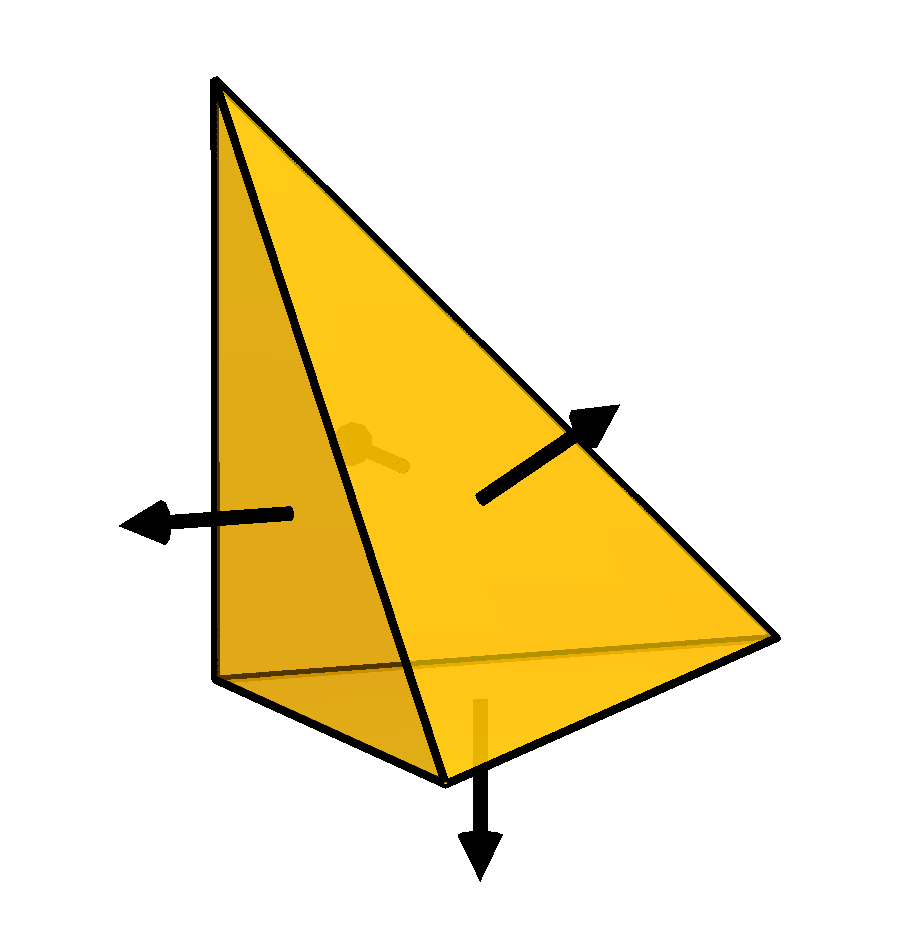
\includegraphics[width=1.3cm]{png/RT1_3d.png}
  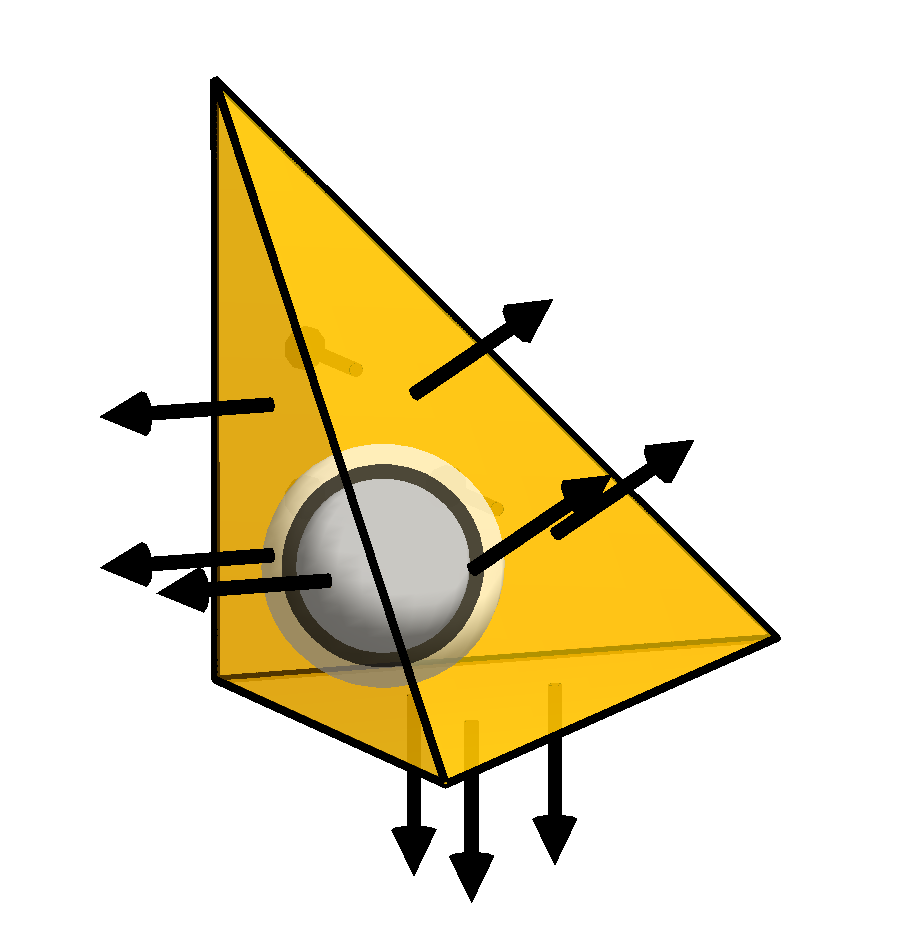
\includegraphics[width=1.3cm]{png/RT2_3d.png} \\
  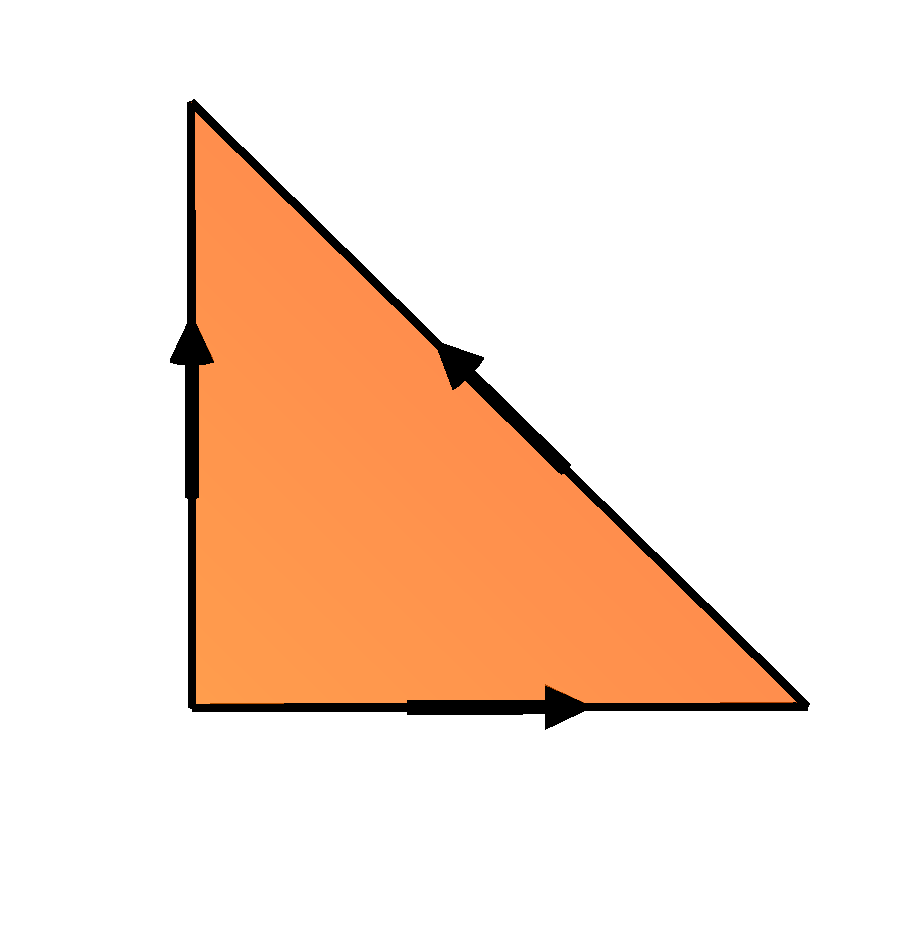
\includegraphics[width=1.3cm]{png/NED1_1_2d.png}
  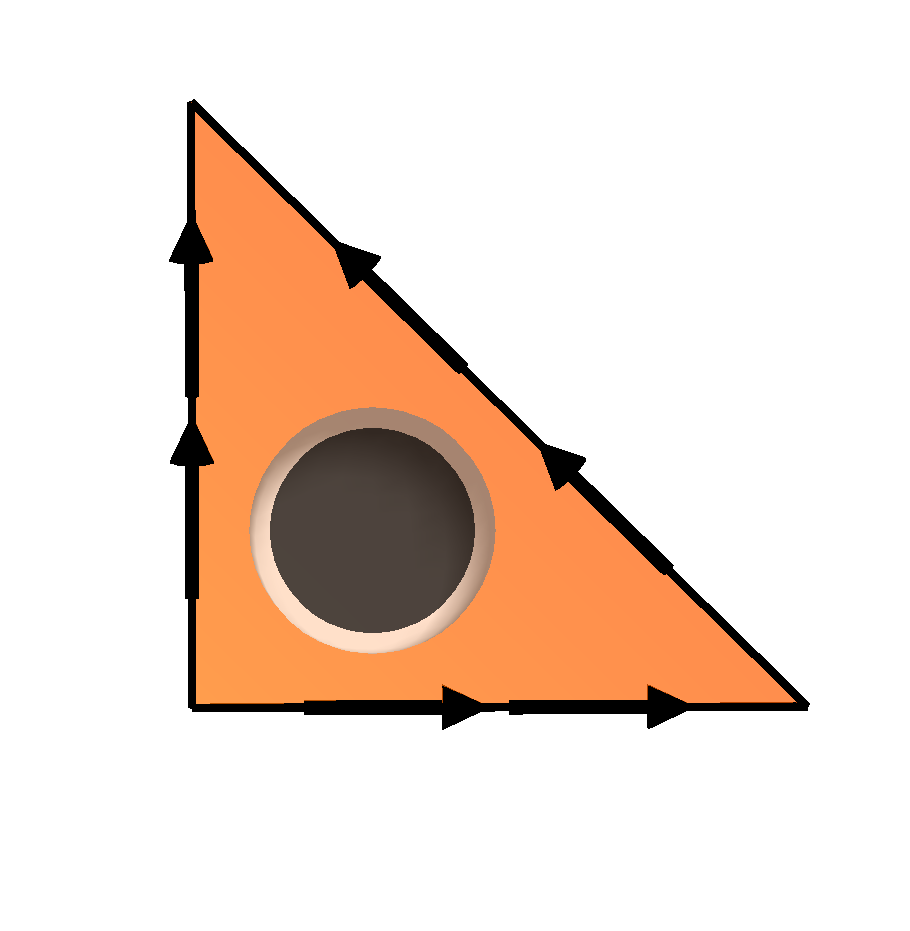
\includegraphics[width=1.3cm]{png/NED1_2_2d.png}
  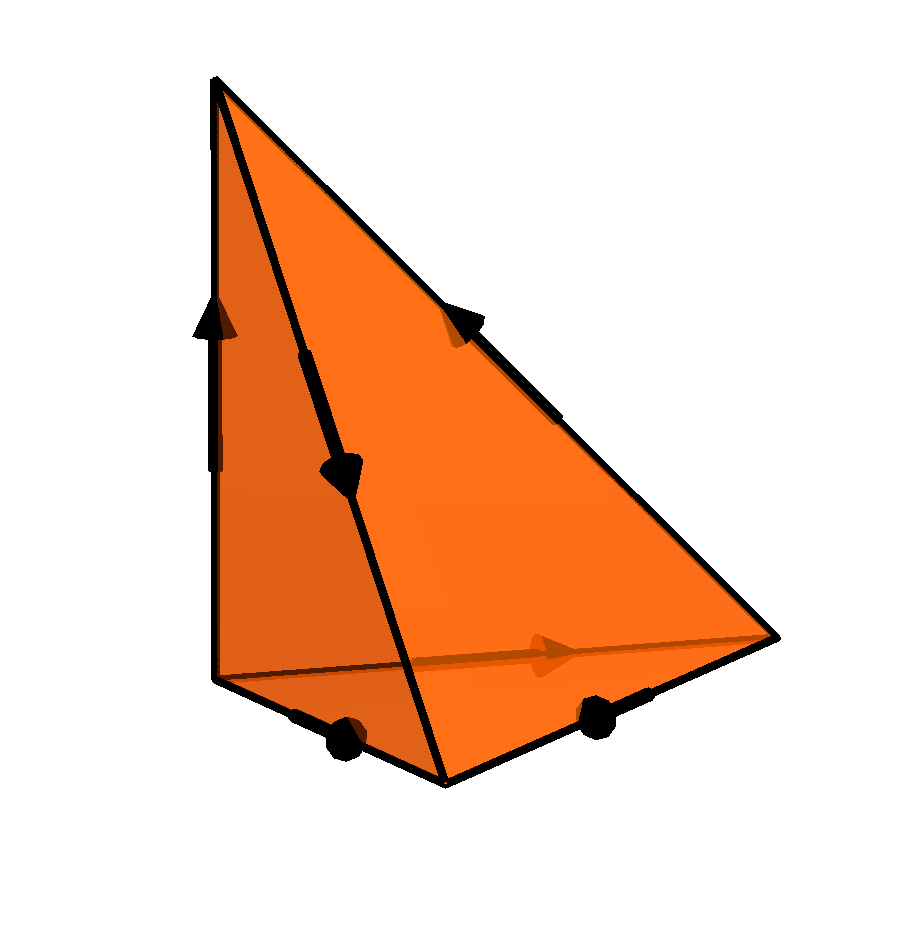
\includegraphics[width=1.3cm]{png/NED1_1_3d.png}
  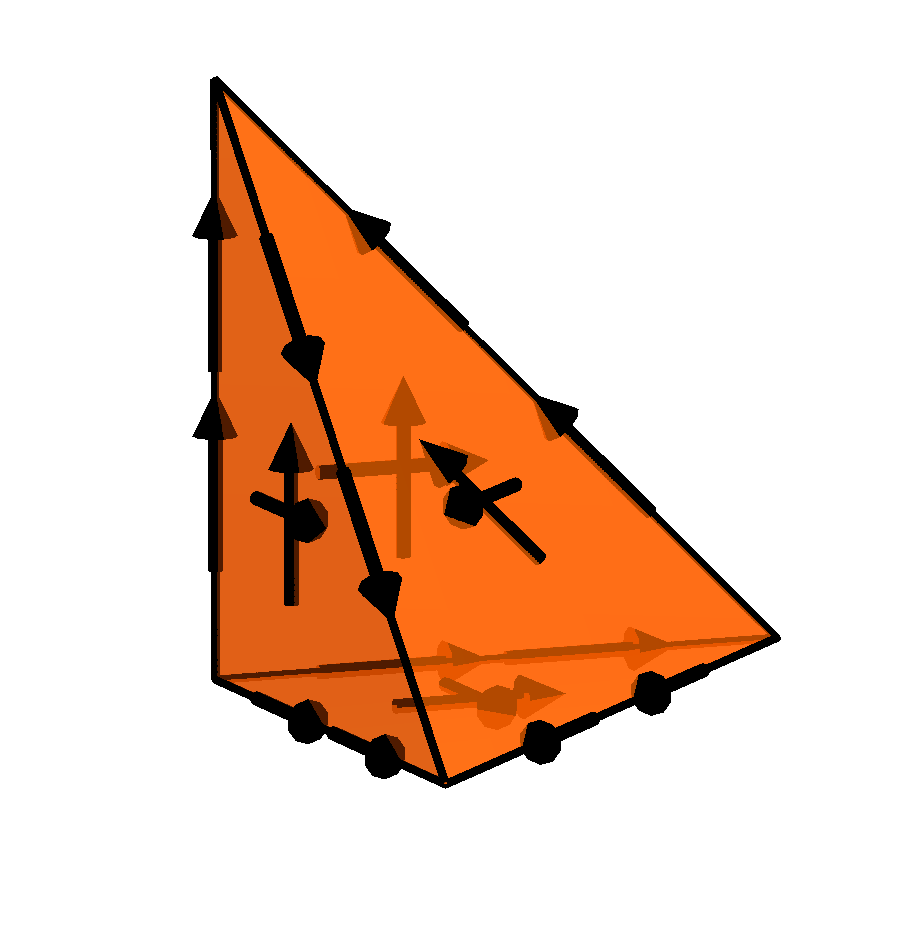
\includegraphics[width=1.3cm]{png/NED1_2_3d.png}
  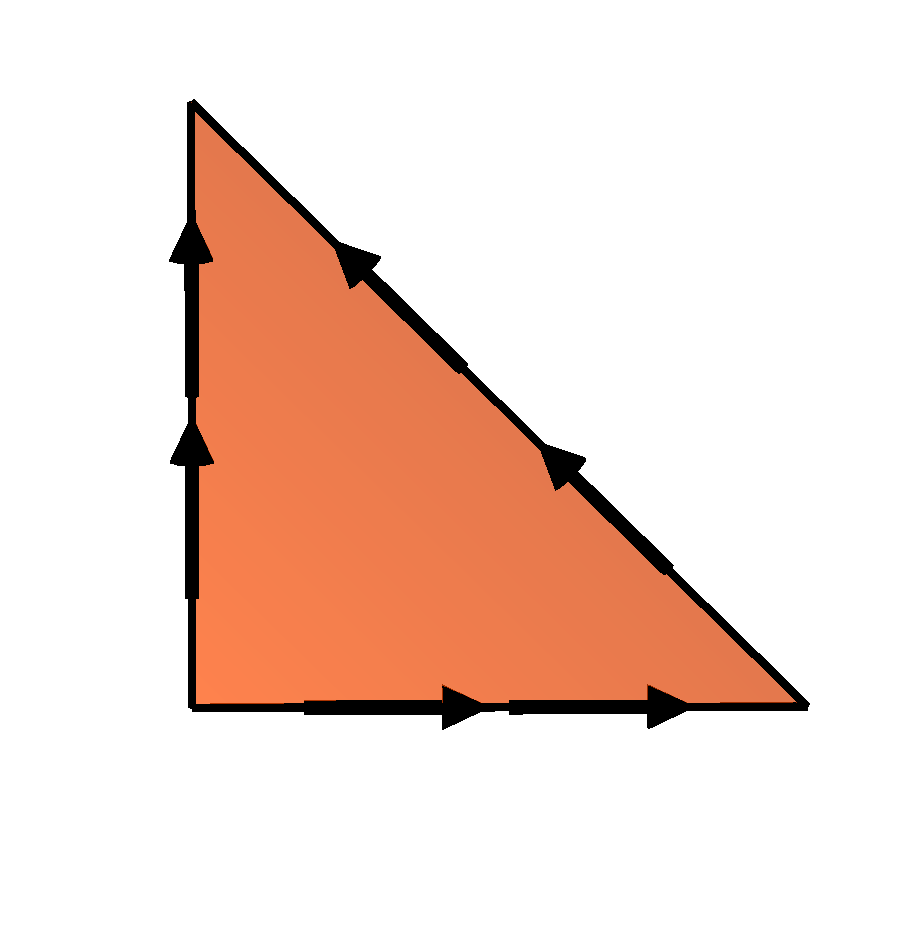
\includegraphics[width=1.3cm]{png/NED2_1_2d.png}
  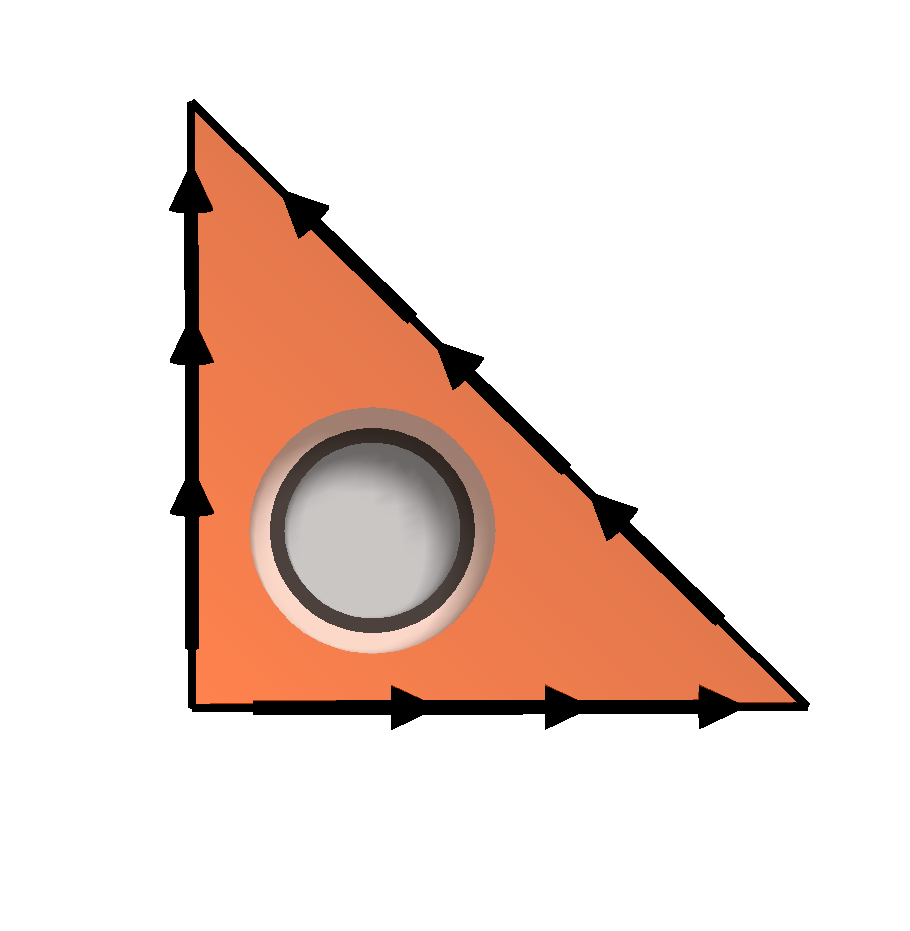
\includegraphics[width=1.3cm]{png/NED2_2_2d.png}
  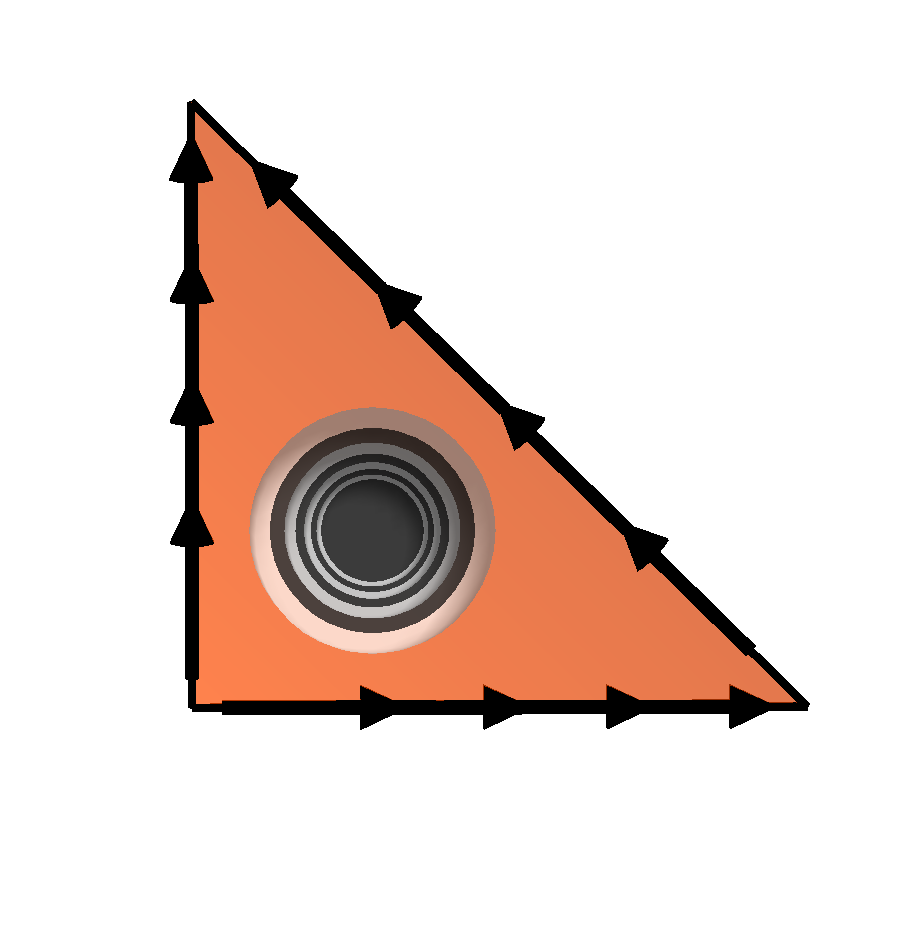
\includegraphics[width=1.3cm]{png/NED2_3_2d.png}
  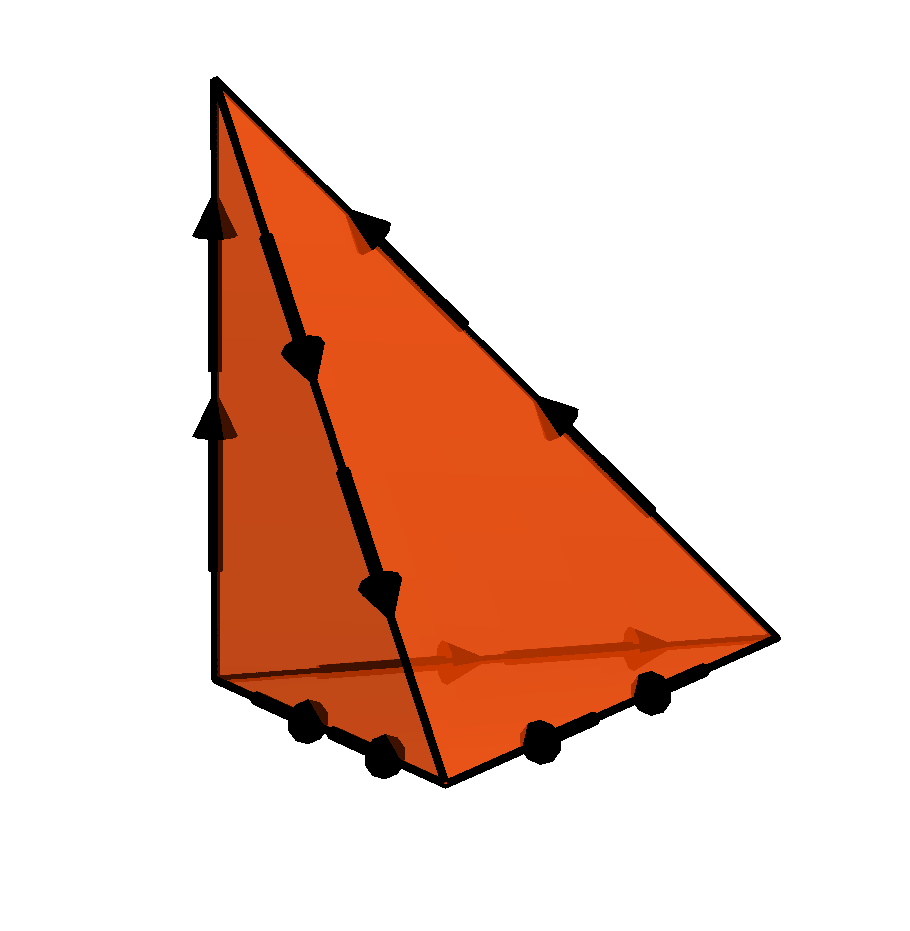
\includegraphics[width=1.3cm]{png/NED2_1_3d.png} \\
  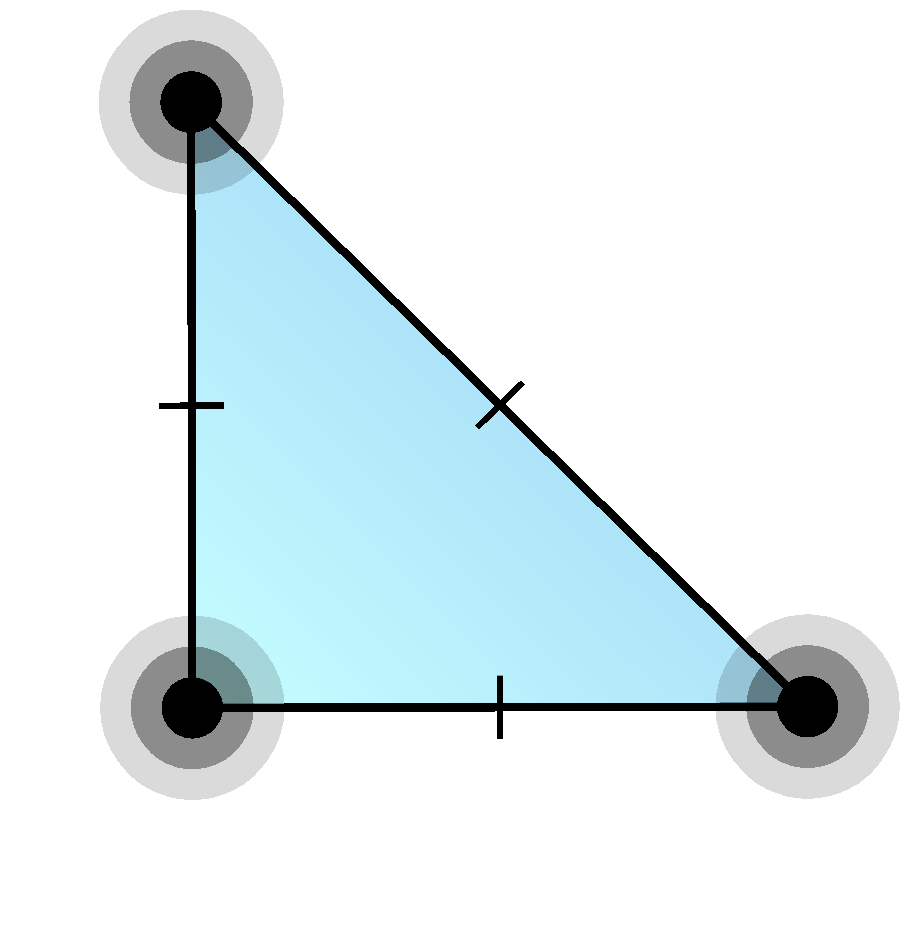
\includegraphics[width=1.3cm]{png/ARG5_2d.png}
  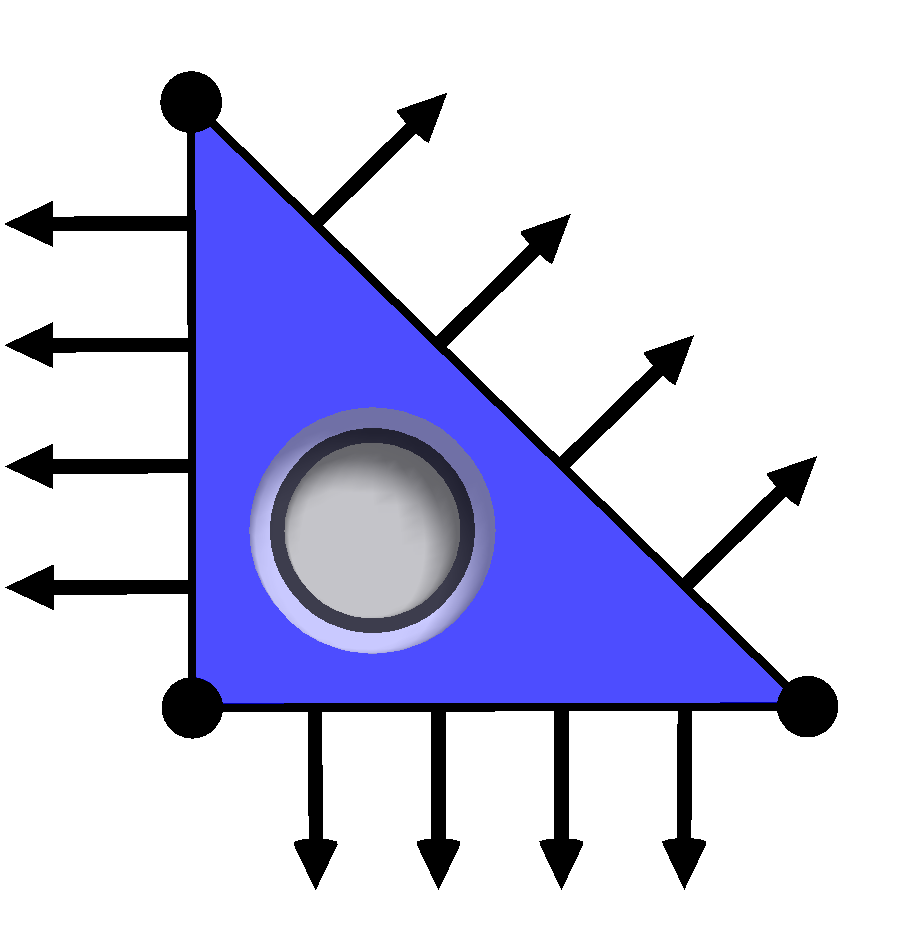
\includegraphics[width=1.3cm]{png/AW_2d.png}
  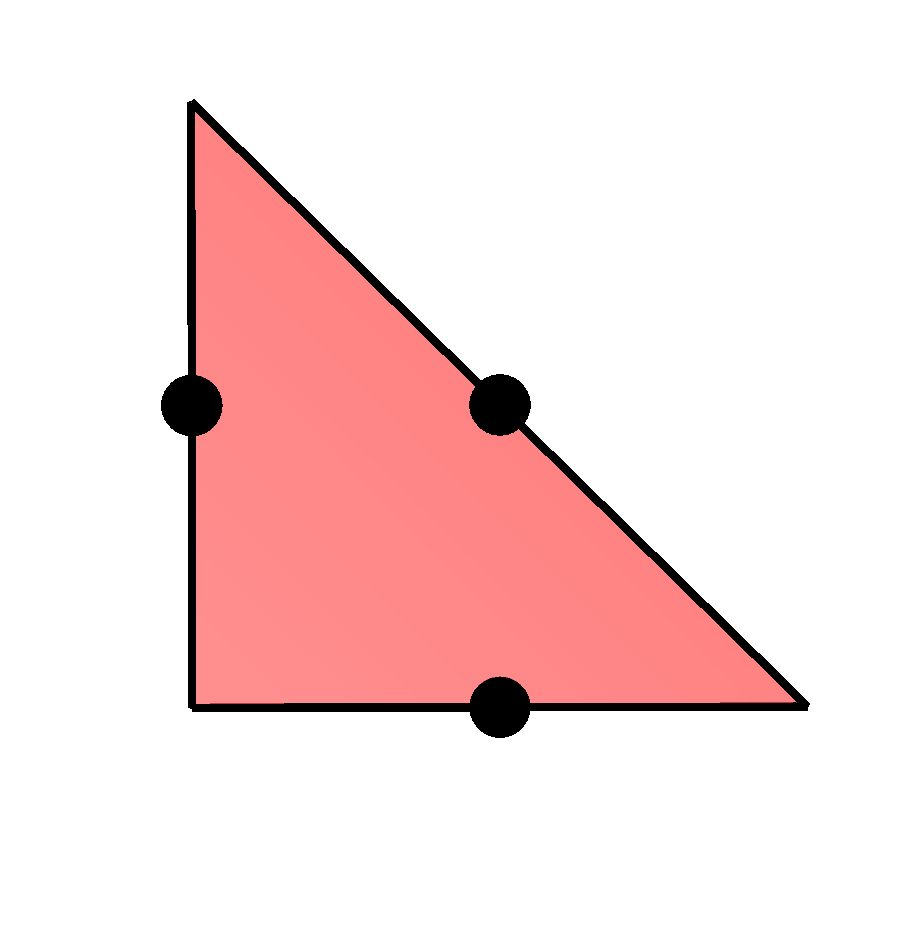
\includegraphics[width=1.3cm]{png/CR1_2d.png}
  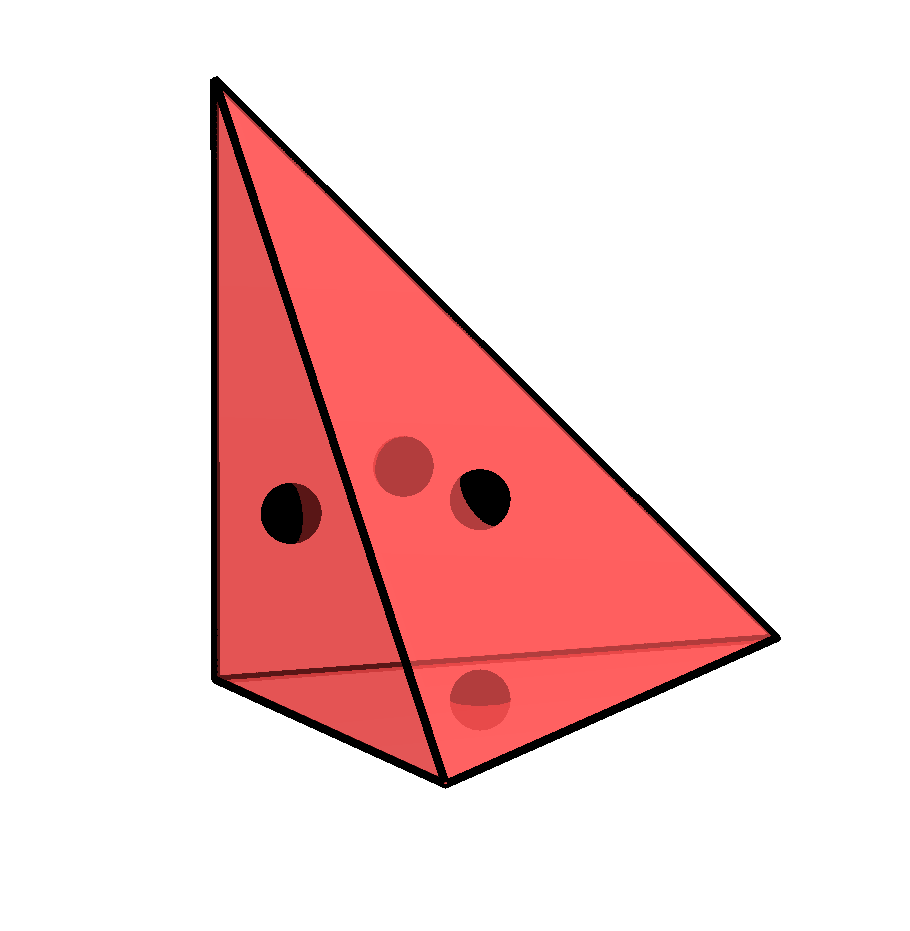
\includegraphics[width=1.3cm]{png/CR1_3d.png}
  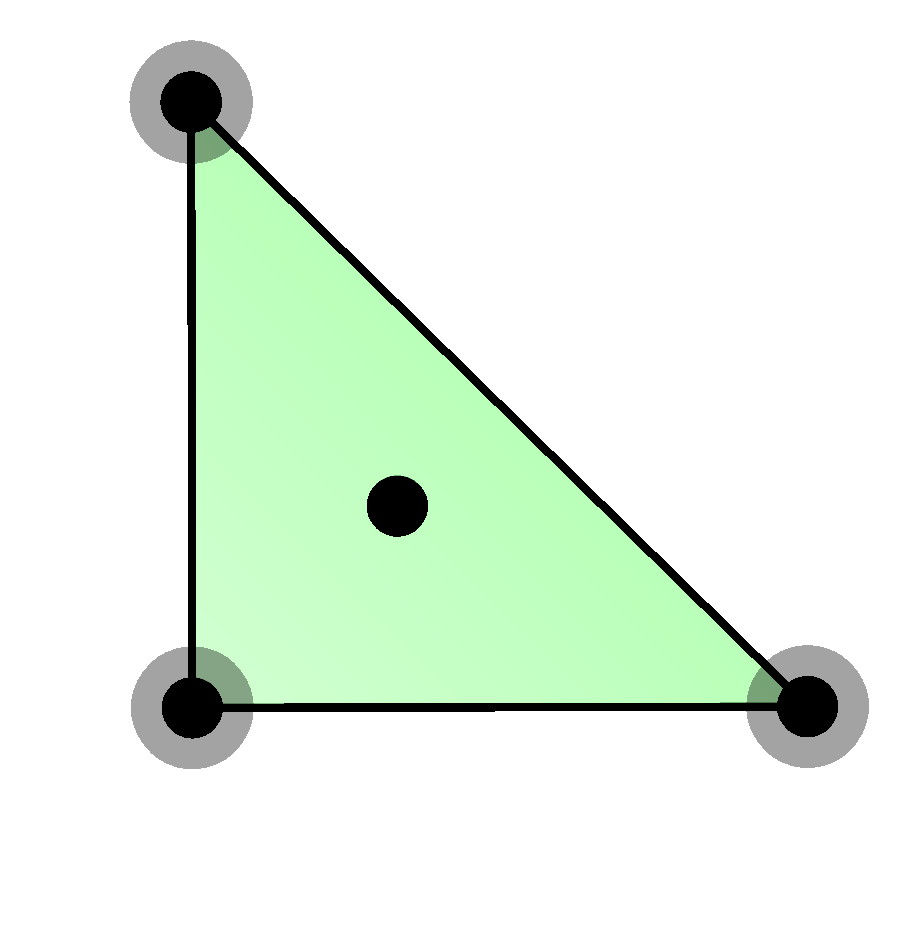
\includegraphics[width=1.3cm]{png/HER_2d.png}
  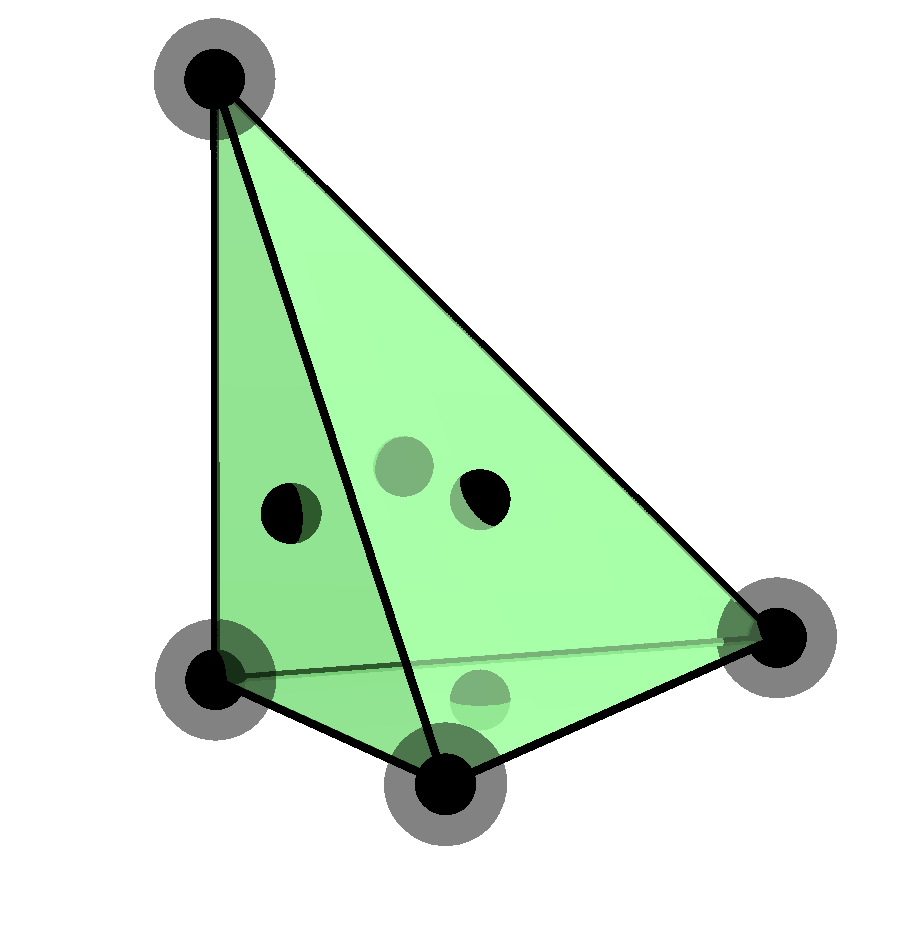
\includegraphics[width=1.3cm]{png/HER_3d.png}
  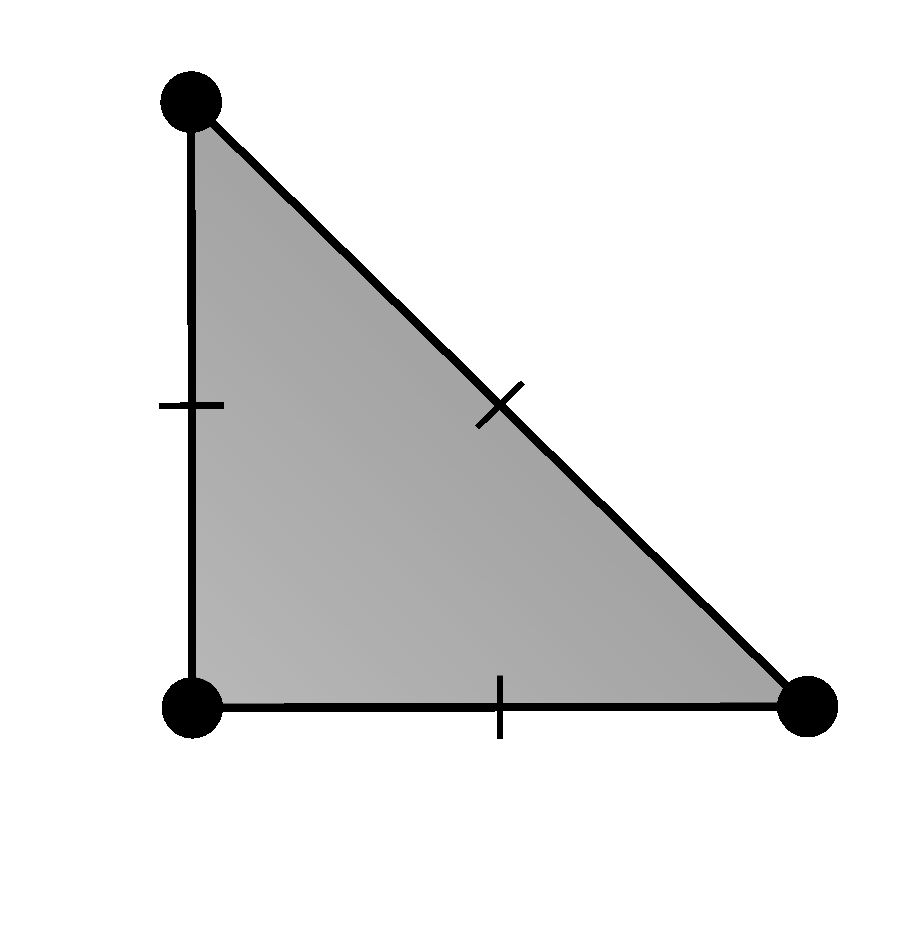
\includegraphics[width=1.3cm]{png/MOR_2d.png}
  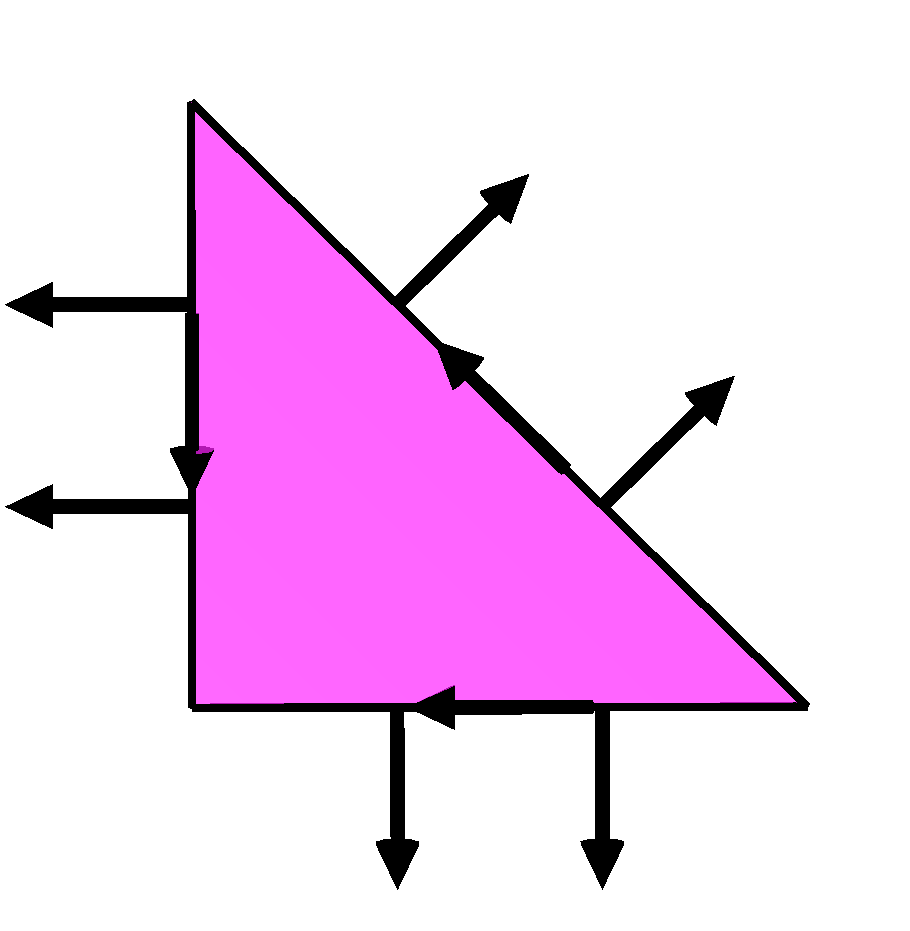
\includegraphics[width=1.3cm]{png/MTW_2d.png}

\end{frame}


\fenicssection{Computing the sparse matrix $A$}

\begin{frame}
  \frametitle{Naive assembly algorithm}

  \begin{tabbing}
    $A = 0$ \\
    \\
    \textbf{for} $i=1,\ldots,N$ \\
    \\
    \tab \textbf{for} $j=1,\ldots,N$ \\
    \\
    \tab \tab $A_{ij} = a(\phi_j, \phi_i)$ \\
    \\
    \tab \textbf{end for} \\
    \\
    \textbf{end for}
  \end{tabbing}

\end{frame}

\begin{frame}
  \frametitle{The element matrix}

  The global matrix $A$ is defined by
  \begin{equation*}
    A_{ij} = a(\phi_j, \phi_i)
  \end{equation*}

  \bigskip

  The \emph{element matrix} $A_T$ is defined by
  \begin{equation*}
    A_{T,ij} = a_T(\phi_j^T, \phi_i^T)
  \end{equation*}

\end{frame}

\begin{frame}
  \frametitle{The local-to-global mapping}

  The global matrix $\iota_T$ is defined by
  \begin{equation*}
    I = \iota_T(i)
  \end{equation*}
  where $I$ is the \emph{global index} corresponding to
  the \emph{local index} i

  \begin{center}
    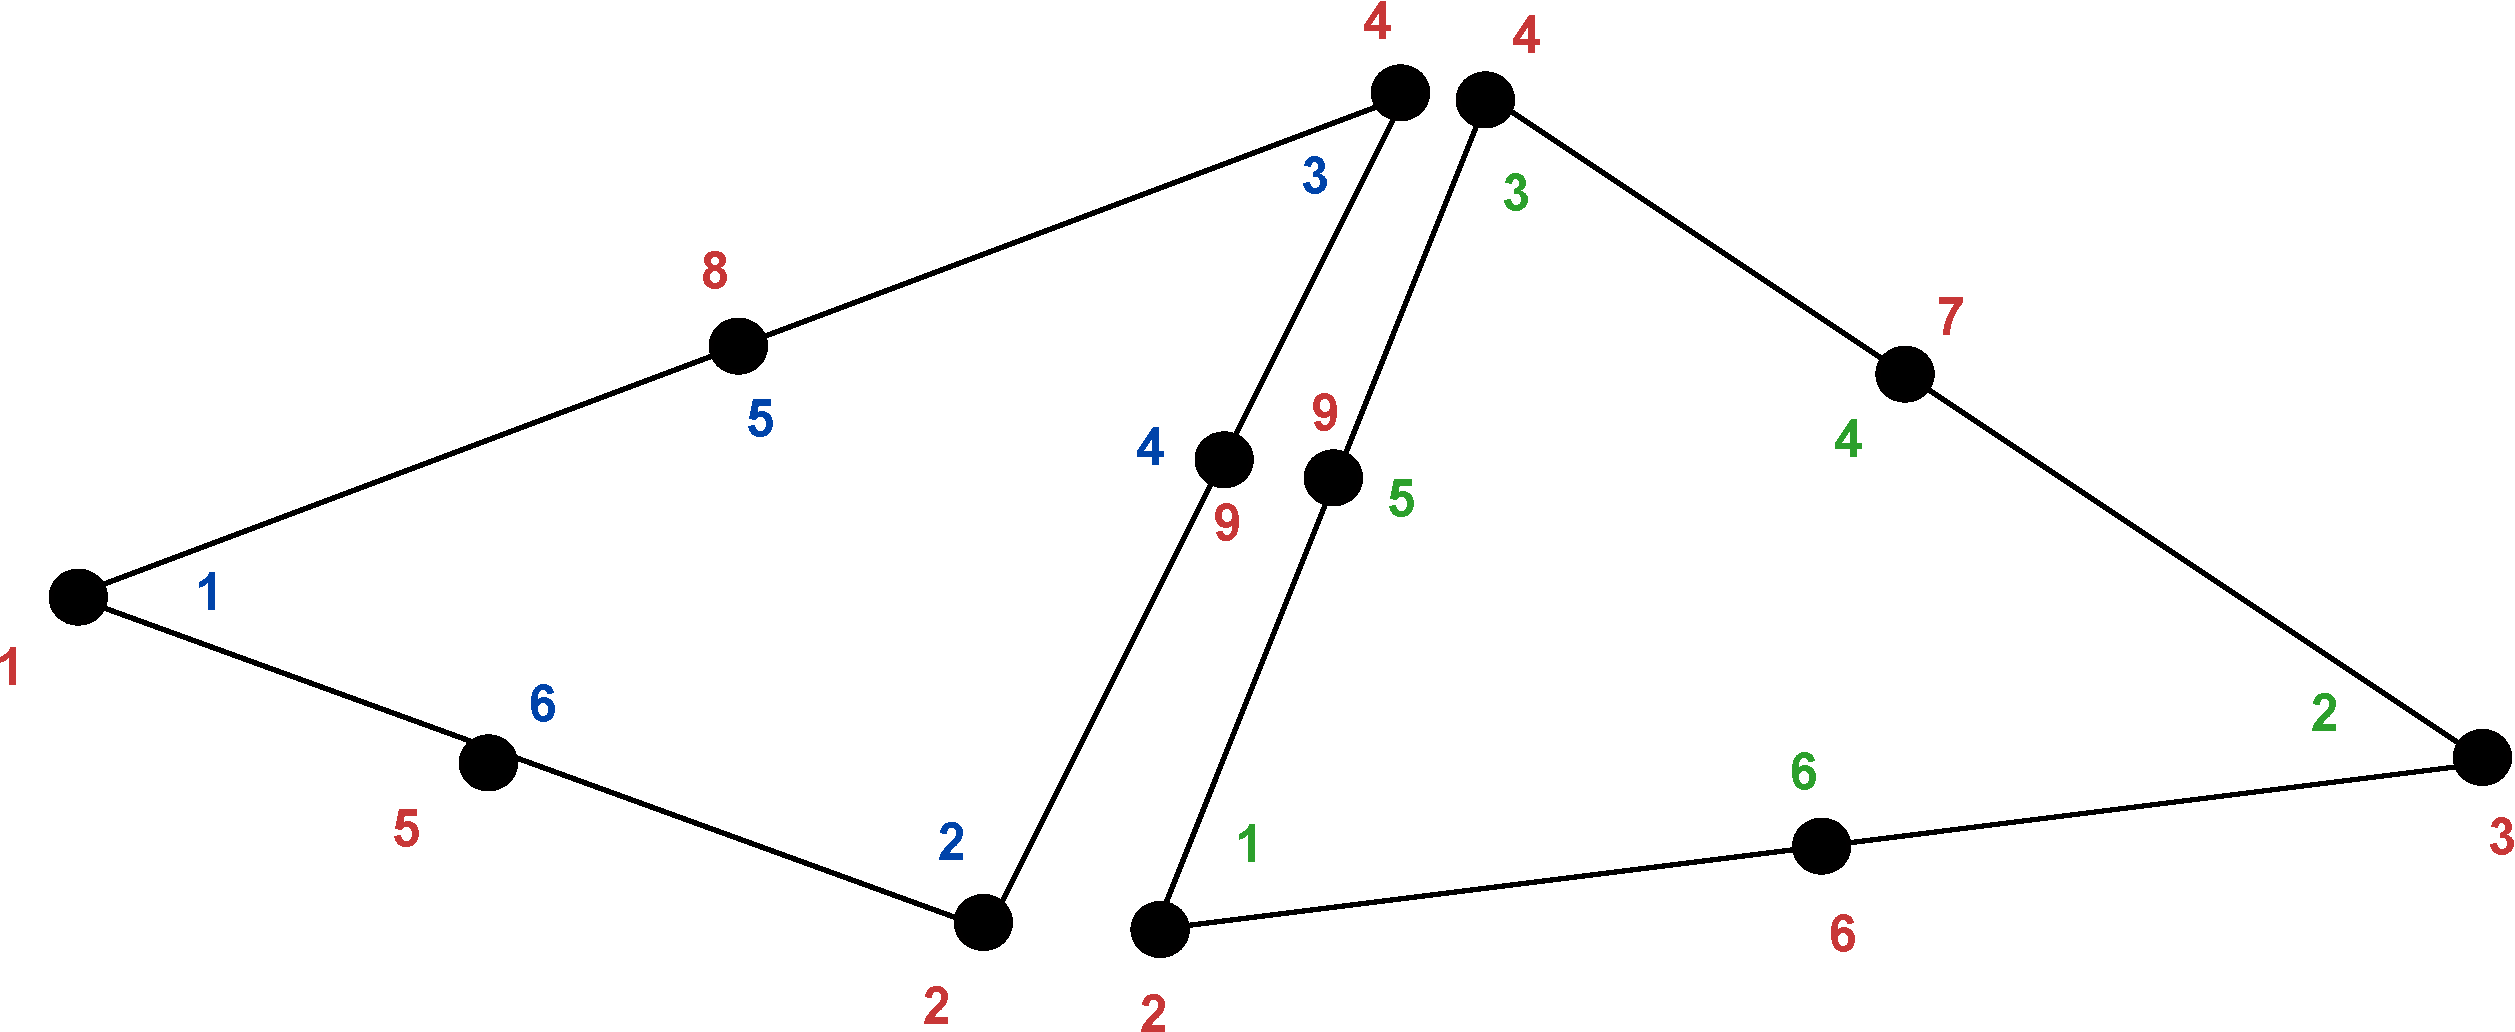
\includegraphics[width=10cm]{pdf/dofmap.pdf}
  \end{center}

\end{frame}

\begin{frame}
  \frametitle{The assembly algorithm}

  \begin{tabbing}
    $A = 0$ \\
    \\
    \textbf{for} $T \in \mathcal{T}$ \\
    \\
    \tab Compute the element matrix $A_T$ \\
    \\
    \tab Compute the local-to-global mapping $\iota_T$ \\
    \\
    \tab Add $A_T$ to $A$ according to $\iota_T$ \\
    \\
    \textbf{end for}
  \end{tabbing}

\end{frame}

\begin{frame}
  \frametitle{Adding the element matrix $A_T$}

  \begin{center}
    \def\svgwidth{\textwidth}
    \import{pdf/}{pdf/insertion.pdf_tex}
  \end{center}

\end{frame}


\fenicssection{Solving $AU = b$}

\begin{frame}
  \frametitle{Direct methods}

  \begin{itemize}
  \item
    Gaussian elimination
    \begin{itemize}
    \item
      Requires $\sim\frac{2}{3}N^3$ operations
    \end{itemize}
  \item
    LU factorization: $A = LU$
    \begin{itemize}
    \item
      Solve requires $\sim\frac{2}{3}N^3$ operations
    \item
      Reuse $L$ and $U$ for repeated solves
    \end{itemize}
  \item
    Cholesky factorization: $A = LL^{\top}$
    \begin{itemize}
    \item
      Works if $A$ is symmetric and positive definite
    \item
      Solve requires $\sim\frac{1}{3}N^3$ operations
    \item
      Reuse $L$ for repeated solves
    \end{itemize}
  \end{itemize}

\end{frame}

\begin{frame}
  \frametitle{Iterative methods}

  Krylov subspace methods
  \begin{itemize}
  \item
    GMRES (Generalized Minimal RESidual method)
  \item
    CG (Conjugate Gradient method)
    \begin{itemize}
    \item
      Works if $A$ is symmetric and positive definite
    \end{itemize}
  \item
    BiCGSTAB, MINRES, TFQMR, \ldots
  \end{itemize}

  Multigrid methods
  \begin{itemize}
  \item
    GMG (Geometric MultiGrid)
  \item
    AMG (Algebraic MultiGrid)
  \end{itemize}

  Preconditioners
  \begin{itemize}
  \item
    ILU, ICC, SOR, AMG, Jacobi, block-Jacobi, additive Schwarz, \ldots
  \end{itemize}

\end{frame}

\begin{frame}
  \frametitle{Which method should I use?}

  Rules of thumb
  \begin{itemize}
  \item
    Direct methods for small systems
  \item
    Iterative methods for large systems
  \item
    Break-even at ca 100--1000 degrees of freedom
  \item
    Use a symmetric method for a symmetric system
    \begin{itemize}
    \item
      Cholesky factorization (direct)
    \item
      CG (iterative)
    \end{itemize}
  \item
    Use a multigrid preconditioner for Poisson-like systems
  \item
    GMRES with ILU preconditioning is a good default choice
  \end{itemize}

\end{frame}

%\begin{frame}
  \frametitle{Current timings (2013--08--09)}

  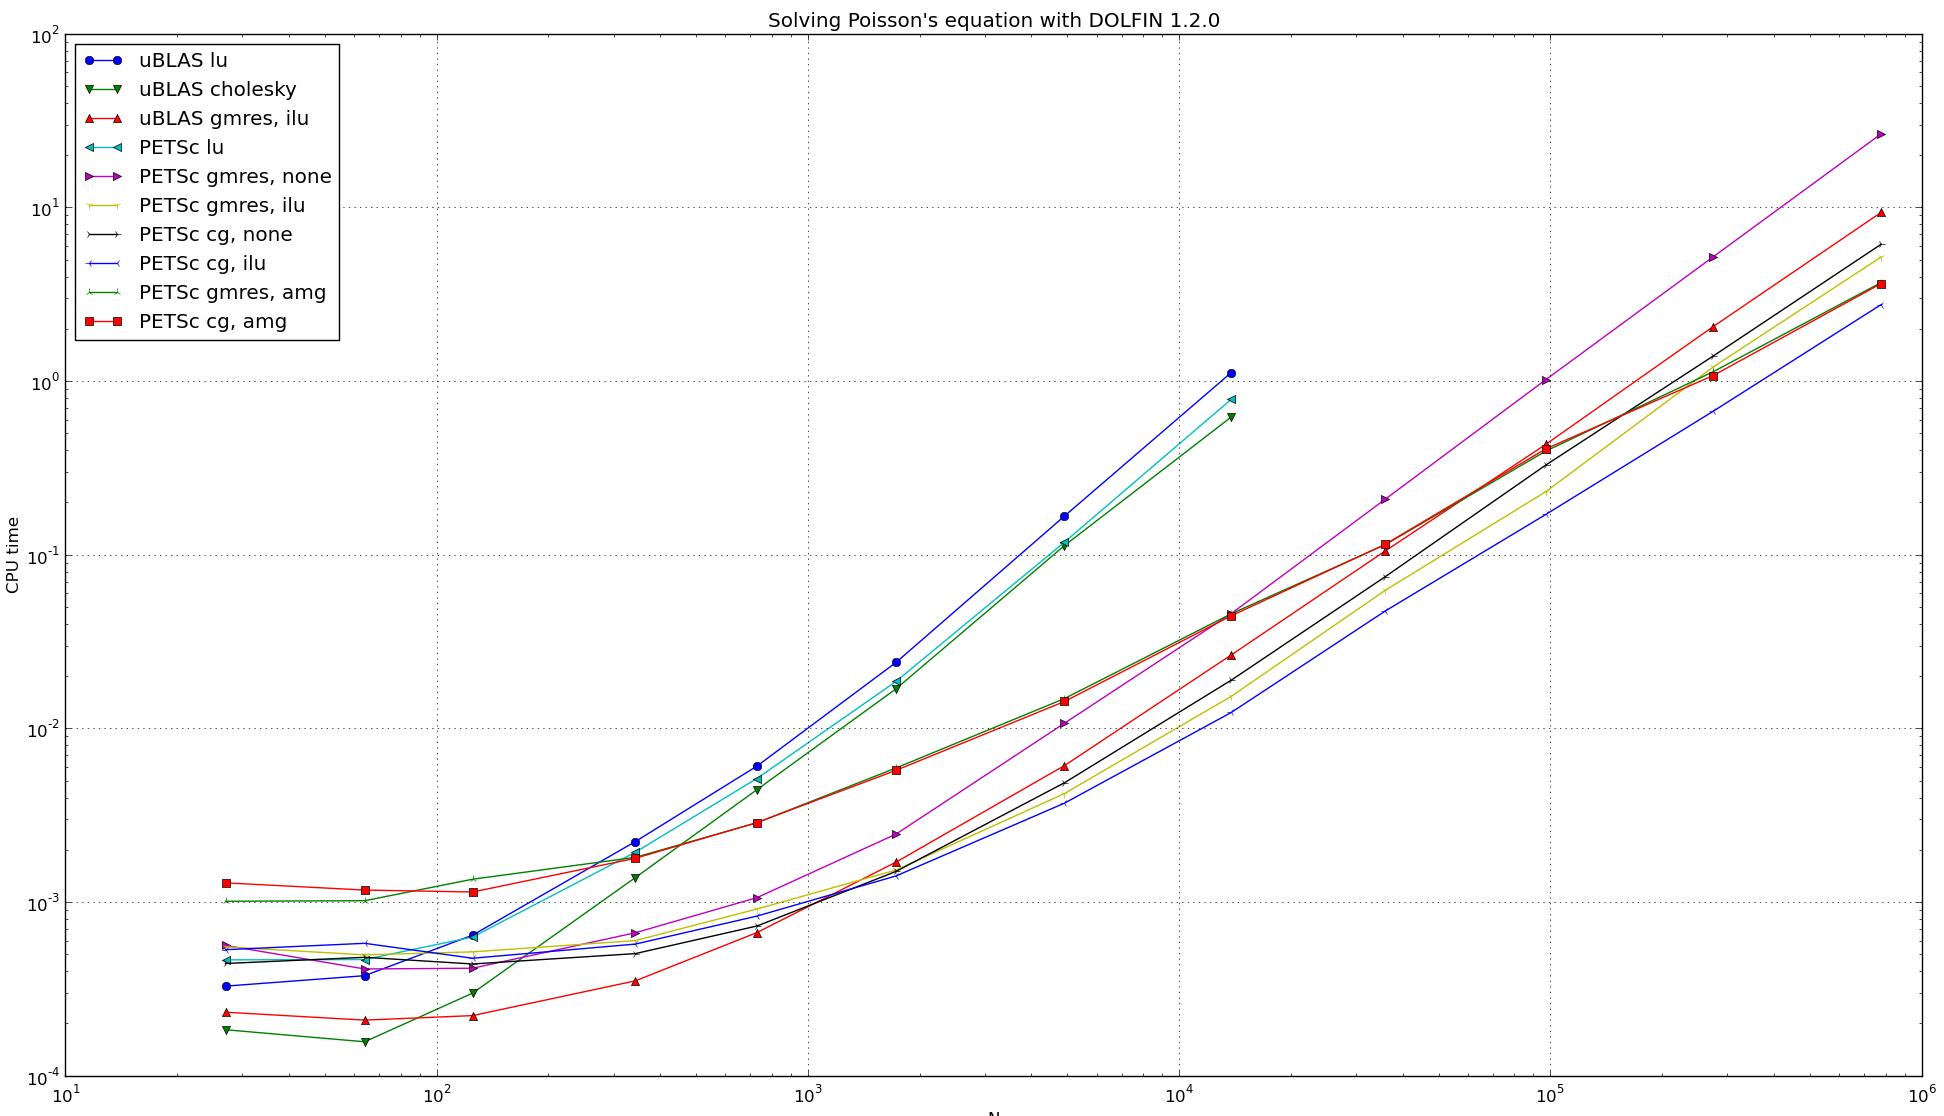
\includegraphics[width=\textwidth]{png/linear_algebra_timings.png}

\end{frame}


% Uncomment if there's a break before the next lecture
%\begin{frame}
  \frametitle{\emph{Homework!}}
  \normalsize

  \begin{columns}

    \begin{column}{0.6\textwidth}

      \begin{itemize}
      \item
        Install FEniCS 1.0.0!
      \item
        Download the FEniCS book!
      \item
        Visit the course web page!
      \end{itemize}

      \vspace{0.5cm}

    \end{column}

    \begin{column}{0.4\textwidth}
      
\includegraphics[height=4cm]{png/fenics_logo.png}
    \end{column}

  \end{columns}

  \large
  \texttt{http://fenicsproject.org/}

  \bigskip

  \texttt{http://fenicsproject.org/pub/course/}

  \vfill

  \small
  \emph{PS: Be alert and ready for the FEniCS challenge(s)\ldots}

\end{frame}


\end{document}
